\chapter{Sufixos}
\markboth{Módulo 1}{}

%\coment{Neste módulo, espera-se que os alunos observem a formação do feminino de adjetivos pátrios terminados em \textbf{-ês}; relacionem o substantivo ao adjetivo formado, conforme os sufixos \textbf{-eza} e \textbf{-esa}; escrevam corretamente as palavras utilizando os sufixos \textbf{-eza} e \textbf{-esa}.}


\colorsec{Habilidades do SAEB}

\begin{itemize}
\item Identificar a ideia central o texto.

\item Localizar informação explícita.

\item Inferir informações implícitas em textos.

\item Inferir o sentido de palavras ou expressões em textos.

\item Reconhecer em textos o significado de palavras derivadas a partir de seus afixos.
\end{itemize}

\colorsec{Habilidades da BNCC}

\begin{itemize}
	\item 
EF04LP08, EF35LP03, EF15LP03, EF35LP04, EF35LP05
\end{itemize}

\conteudo{
\textbf{Palavras terminadas em -ês, -esa, -ez, -eza}\bigskip

\noindent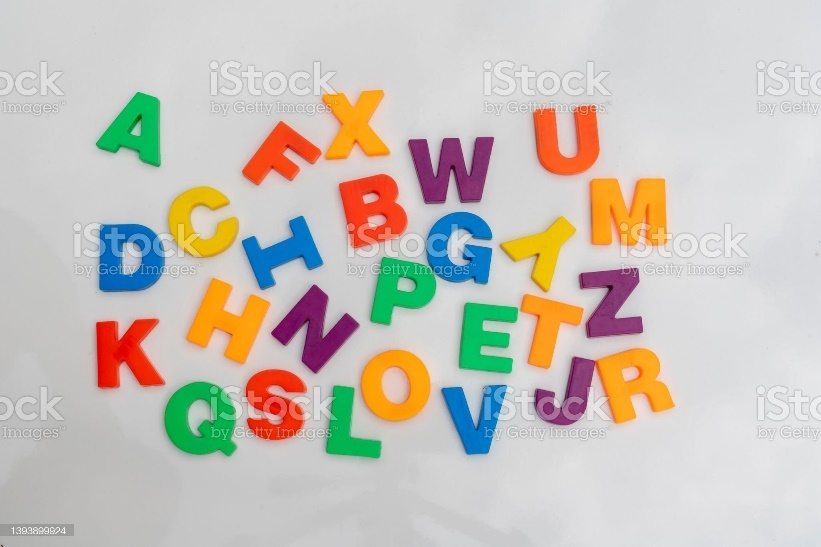
\includegraphics[width=\textwidth]{media/image1.jpeg}

Na língua portuguesa, há palavras que terminam com \textbf{-eza} e
palavras que terminam com \textbf{-esa}. Esses sufixos (terminações) são
pronunciados do mesmo modo, mas há regras próprias que devem ser
seguidas em seu uso. Observe os quadros a seguir.

\begin{myquote}
O sufixo \textbf{-eza} transforma adjetivos em substantivos abstratos.

Exemplos: fraco -- fraqueza; delicado -- delicadeza; firme -- firmeza.
\end{myquote}

\begin{myquote}
O sufixo \textbf{-esa} é usado para formar adjetivos pátrios no
feminino: (holandês -- holandesa; francês -- francesa; inglês --
inglesa; chinês -- chinesa; príncipe -- princesa; duque -- duquesa;
camponês -- camponesa; burguês -- burguesa).
\end{myquote}

As palavras terminadas em \textbf{-esa} fazem parte da classe gramatical
dos \textbf{adjetivos} e as palavras terminadas em \textbf{-eza} fazem
parte da classe gramatical dos \textbf{substantivos}.
}

\colorsec{Atividades}

Leia, agora, o início do conto \textbf{A roupa nova do imperador}, do 
escritor Hans Christian Andersen. Nesse texto, você vai conhecer a 
história de um imperador muito vaidoso, que gostava de ter muitas
roupas, mas que foi enganado por dois falsos tecelões.

%\coment{Oriente os alunos a realizar, primeiramente, leitura silenciosa do texto, seguida de leitura em voz alta. Essa estratégia de leitura possibilita que o aluno desenvolva fluência leitora, facilitando a compreensão global do texto lido. As atividades introdutórias são de compreensão do texto e têm a finalidade de desenvolver habilidades de localizar informações, realizar simples inferências, deduzir significados de termos do texto e inferir o tempo em que ocorre a narrativa.}

\begin{quote}
\textbf{A roupa nova do imperador}

Há muito, muito tempo, vivia em um reino distante um imperador
vaidosíssimo. Seu único interesse eram as roupas. Pensava apenas em
trocar de roupas, várias vezes ao dia; desfilava vestes belíssimas,
luxuosas e muito caras para a corte. Um belo dia, chegaram à capital do
reino dois pilantras, muito habilidosos em viver às custas do próximo.

Assim que os dois souberam da fraqueza do imperador por belas roupas,
espalharam a notícia de que eles eram especialistas em tecer um pano
único no mundo, de cores e padrões deslumbrantes. E --- o mais
impressionante, segundo eles: as roupas confeccionadas com aquele tecido
tinham o poder de serem invisíveis para as pessoas tolas, ou que
ocupassem um cargo sem merecê-lo. {[}...{]}

\fonte{Hans Christian Andersen. Domínio Público. A roupa nova do imperador. Disponível
em: www.dominiopublico.gov.br/download/texto/me000589.pdf.
Acesso em: 24 abr. 2023.}
\end{quote}

\begin{figure}[htpb!]
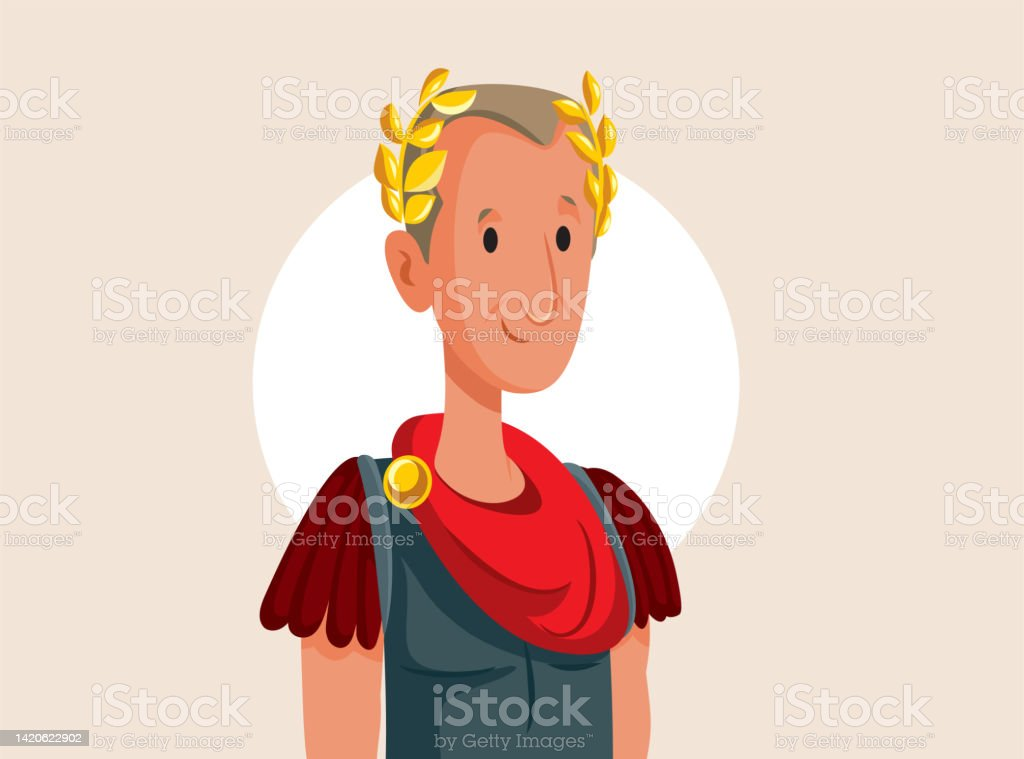
\includegraphics[width=\textwidth]{media/image2.jpeg}
\end{figure}

%\begin{tabular}{ll}
%\textbf{Glossário} & \mbox{}\\
%Pilantra & pessoa desonesta.\\
%\end{tabular}

\pagebreak
\num{1} Onde o imperador vivia?

\reduline{O imperador vivia em um reino distante.\hfill}
\linhas{2}

\num{2} Qual era o único interesse do imperador?

\reduline{O único interesse do imperador eram as roupas.\hfill}
\linhas{2}

\num{3} Qual foi a notícia que os dois pilantras espalharam 
ao saber da fraqueza do imperador?

\reduline{Eles espalharam a notícia de que eram especialistas
em tecer um pano único no mundo, de cores e padrões deslumbrantes. E que
as roupas confeccionadas com aquele tecido tinham o poder de serem
invisíveis para as pessoas tolas, ou que ocupassem um cargo sem
merecê-lo.\hfill}
\linhas{2}

\num{4} Releia um trecho do conto e observe os termos destacados.

\begin{quote}
Assim que os dois souberam da \textbf{fraqueza} do imperador por
\textbf{belas} roupas, espalharam a notícia de que eles eram
especialistas em tecer um pano único no mundo, de cores e padrões
deslumbrantes.
\end{quote}

\begin{escolha}
\item
A que classe de palavras pertence o termo \textbf{belas}?

\reduline{O termo \textbf{belas} pertence à classe dos adjetivos.\hfill}

\item
A que classe de palavras pertence a palavra \textbf{fraqueza}?

\reduline{A palavra \textbf{fraqueza} pertence à classe dos substantivos.\hfill}
\end{escolha}

\num{5} Complete as frases com os \textbf{adjetivos} do quadro.

\begin{mdframed}[linewidth=2pt,linecolor=salmao,roundcorner=10pt]
\textbf{macia}\hfill \textbf{fraco}\hfill \textbf{gentil}\hfill
\end{mdframed}

\begin{escolha}
\item O resfriado que peguei me deixou muito \reduline{fraco\hfill}.

\item Ela é uma pessoa muito \reduline{gentil\hfill}.

\item A toalha do hotel era muito \reduline{macia\hfill}.
\end{escolha}

\num{6} Transforme os adjetivos que você usou para completar as frases
da atividade anterior em \textbf{substantivos}.

\reduline{Fraqueza\hfill}

\reduline{gentileza\hfill}

\reduline{maciez.\hfill}

\num{7} O escritor do conto que você leu, Hans Christian Andersen, nasceu na Dinamarca.

\begin{escolha}
\item Um rapaz que nasce na Dinamarca é \reduline{dinamarquês\hfill}.

\item Uma moça que nasce na Dinamarca é \reduline{dinamarquesa\hfill}.
\end{escolha}\enlargethispage{\baselineskip}

\num{8} Observe as bandeiras a seguir e leia o nome dos respectivos países a que elas correspondem.

\begin{figure}[htpb!]

\includegraphics[width=.3\textwidth]{media/image3.png}

\includegraphics[width=.3\textwidth]{media/image4.png}

\includegraphics[width=.3\textwidth]{media/image5.jpeg}
\caption{Portugal, Holanda e Japão}
\end{figure}

\pagebreak
Escreva na tabela o nome do país de origem e as nacionalidades correspondentes. Siga o exemplo.

\begin{longtable}[]{@{}lll@{}}
\toprule
\begin{minipage}[b]{0.32\columnwidth}\raggedright\strut
\textbf{País de origem}\strut
\end{minipage} & \begin{minipage}[b]{0.32\columnwidth}\raggedright\strut
\textbf{Nacionalidade masculina}
\strut
\end{minipage} & \begin{minipage}[b]{0.32\columnwidth}\raggedright\strut
\textbf{Nacionalidade feminina }
\strut
\end{minipage}\tabularnewline
\midrule
\endhead
\begin{minipage}[t]{0.32\columnwidth}\raggedright\strut
França\strut
\end{minipage} & \begin{minipage}[t]{0.32\columnwidth}\raggedright\strut
francês
\strut
\end{minipage} & \begin{minipage}[t]{0.32\columnwidth}\raggedright\strut
francesa
\strut
\end{minipage}\tabularnewline
\rosa{Portugal} & \rosa{português} & \rosa{portuguesa}\tabularnewline
\rosa{Holanda} & \rosa{holandês} & \rosa{holandesa}\tabularnewline
\rosa{Japão} & \rosa{japonês} & \rosa{japonesa}\tabularnewline
\bottomrule
\end{longtable}

\num{9} Em relação à terminação das palavras que você escreveu, o que é possível
concluir sobre a grafia delas?

\reduline{As palavras terminadas em \textbf{-ês}, quando flexionadas no feminino, terminam em \textbf{-esa}.\hfill}
%\linhas{3}

\num{10} No caça-palavras, encontre palavras femininas de nacionalidades dos
países de origem que estão no quadro. Em seguida, escreva as palavras
encontradas na linhas.

\begin{mdframed}[linewidth=2pt,linecolor=salmao,roundcorner=10pt]
\textbf{Holanda}\hfill \textbf{Albânia}\hfill \textbf{Escócia}\hfill \textbf{Finlândia}\hfill \textbf{Inglaterra}
\end{mdframed}

\begin{minipage}{.5\textwidth}
\begin{longtable}[]{@{}llllllllllll@{}}
\toprule
T & N & L & H & E & A & C & L & V & N & E & S\tabularnewline
\midrule
\endhead
I & W & G & O & A & M & E & I & E & A & D & N\tabularnewline
H & O & L & A & N & D & E & S & A & L & O & V\tabularnewline
I & E & I & F & N & T & R & D & O & T & E & P\tabularnewline
T & F & I & N & L & A & N & D & E & S & A & E\tabularnewline
I & O & N & I & T & S & U & T & C & L & V & I\tabularnewline
E & R & G & E & I & T & L & O & B & E & T & T\tabularnewline
E & O & L & W & N & S & C & A & H & E & A & P\tabularnewline
K & D & E & L & E & E & N & H & E & W & A & N\tabularnewline
I & R & S & S & S & E & T & L & E & R & H & U\tabularnewline
I & E & A & A & S & P & I & I & H & N & H & A\tabularnewline
O & S & I & A & L & U & D & T & S & A & T & I\tabularnewline
\bottomrule
\end{longtable}
\end{minipage}\hspace{3cm}
\begin{minipage}{.3\textwidth}
\linhas{5}
\end{minipage}

\colorsec{Treino}

\num{1} Observe a bandeira da Inglaterra. %(Fácil)


\begin{figure}[htpb!]
\centering

\includegraphics[width=.5\textwidth]{media/image6.jpeg}
\end{figure}

Uma mulher e um homem que nascem na Inglaterra são, respectivamente

\begin{multicols}{2}
\begin{escolha}
\item ingleza e inglezo.

\item inglaterra e inglaterro.

\item inglaterrana e inglaterrano.

\item inglesa e inglês.
\end{escolha}
\end{multicols}

\num{2} Analise um trecho de um dos contos populares tradicionais africanos, ``Oxóssi''.
%(Médio) 

\begin{quote}
\textbf{Oxóssi}

Olofin era um rei africano da terra de Ifé, lugar de origem de todos os
iorubás.

Cada ano, na época da colheita, Olofin comemorava, em seu reino, a Festa
dos Inhames.

Ninguém no país podia comer dos novos inhames antes da festa. Chegando o
dia, o rei se instalava no pátio do seu palácio. Suas mulheres sentavam 
à sua direita, seus ministros atrás dele, agitando leques e 
espanta-moscas, e os tambores soavam para saudá-lo.

As pessoas reunidas comiam inhame pilado e bebiam vinho de palma. Elas
comemoravam e brincavam.

%Fábia e Felipe: padronizando textos que o autor extraiu dessa coleção de alfabetização: Nome da autora seguido de ``e outros'' (para evitar et al). Título do texto usado. Título do livro, com volume e subtítulo. Verifiquem se essa padronização agrada. 

\fonte{Ana Rosa Abreu e outros autores. Oxóssi. Alfabetização, Vol.2: contos, fábula, lendas e mitos. Disponível em:
www.dominiopublico.gov.br/download/texto/me000589.pdf.
Acesso em: 24 abr. 2023.}
\end{quote}

\pagebreak
No trecho de ``Oxóssi'', os tambores soavam com o objetivo de

\begin{escolha}
\item comemorar a colheita dos inhames.

\item permitir o início do jantar.

\item fazer homenagem ao rei durante a festa.

\item acompanhar os ministros na festa.
\end{escolha}

\num{3} Leia o texto a seguir. %(Difícil)

\begin{quote}
\textbf{Pequenas agricultoras}

As formigas cortadeiras cultivam seu próprio jardim dentro do
formigueiro. {[}...{]}

Formigas cortadeiras, como as saúvas, são especializadas em cultivar
fungos. Os pedacinhos de folhas que elas cortam são levados para câmaras
especiais dentro dos formigueiros onde servirão como base para crescimento
desses fungos. Essas câmaras são chamadas pelos cientistas de ``jardins de
fungos''. Mas cortar e carregar todas aquelas folhinhas é só o início de um
trabalho minucioso de cultivo.

\fonte{Vinícius São Pedro. Ciência Hoje das Crianças. Pequenas agricultoras. Disponível em:
http://chc.org.br/artigo/pequenas-agricultoras/. Acesso em: 24 abr.
2023.}
\end{quote}

O texto ``Pequenas agricultoras'' tem a finalidade de informar sobre

\begin{escolha}
\item a importância dos fungos no formigueiro.

\item o trabalho das formigas cortadeiras.

\item o modo de cultivar um jardim com formigas.

\item o trabalho de agricultores especializados.
\end{escolha}
%As alterações acima têm a finalidade de deixar o texto das alternativas com o mesmo tamanho. Nunca falamos sobre isso, Fábia e Felipe, mas, sempre que escrevi material didático, recebi essa orientação das editoras, para evitar induzir os alunos ao erro ou ao acerto. 



\chapter{Cartas}
\markboth{Módulo 2}{}

%\coment{Neste módulo, os alunos farão leitura de cartas, de modo a aperfeiçoar a compreensão de textos desse gênero do campo da vida cotidiana. As atividades terão foco na identificação do objetivo da produção -- no que se refere à incitação de seus autores e eventuais argumentos para justificá-la -- e de elementos da organização textual, assim como a exploração da linguagem empregada.}


\colorsec{Habilidades do SAEB}

\begin{itemize}
\item Reconhecer diferentes gêneros textuais.

\item Identificar elementos constitutivos de textos narrativos.

\item Identificar as marcas de organização de textos dramáticos.

\item Analisar os efeitos de sentido de verbos de enunciação.
\end{itemize}


\colorsec{Habilidades da BNCC}

\begin{itemize}
	\item
EF04LP10, EF04LP14, EF04LP27, EF35LP24, EF35LP26.
\end{itemize}

\conteudo{
\textbf{Cartas}

Quando o celular e a internet ainda não eram tão populares, um dos meios
mais utilizados para comunicação entre pessoas que estavam distantes uma 
da outra era a carta.

Sempre houve quem gostasse de escrever cartas. E, ainda hoje,
mesmo com tantas outras possibilidades, existem aqueles que fazem
questão de escrever cartas aos amigos, parentes, etc.

A carta pessoal é uma mensagem que pode ser escrita à mão ou digitada. É
um texto escrito para alguém, ou seja, um destinatário, com o objetivo
de estabelecer contato com ele. A linguagem utilizada costuma ser informal.

No verso do envelope, devem ser escritas as informações de quem envia a 
carta, o \textbf{remetente}; na frente, ficam registrados os dados de
quem receberá a carta, o \textbf{destinatário}.
As informações de destinatário servem para que o serviço de Correios
entregue a carta no local correto. Para isso, ambas as informações devem
conter nome, endereço completo (rua, número, bairro, cidade e estado) e
CEP (código de endereçamento postal).

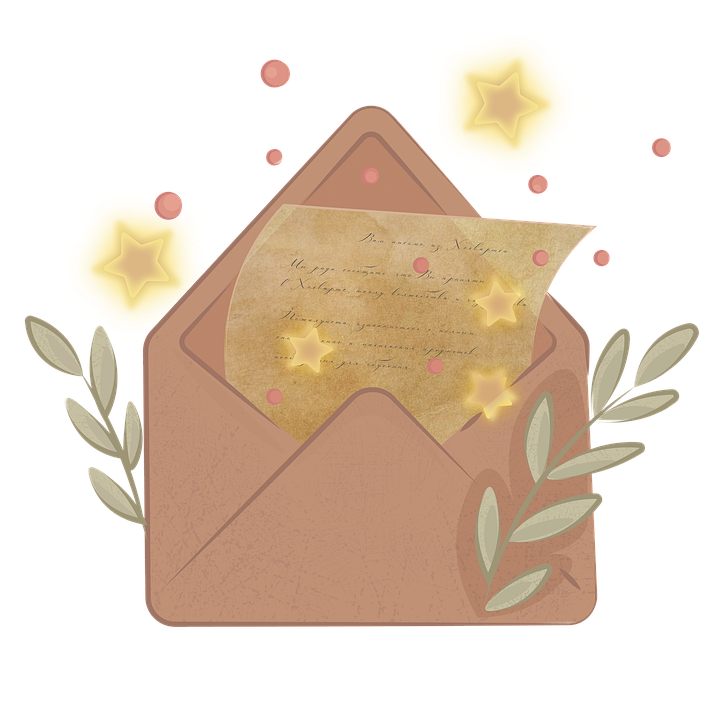
\includegraphics[width=\textwidth]{media/image7.png}

O conteúdo da carta deve vir em uma folha dentro do envelope, que deverá
ser lida apenas pelo destinatário a quem a carta foi endereçada.

Hoje em dia, entretanto, há outros meios de manter diálogo com pessoas 
distantes, como o celular, os aplicativos de mensagens instantâneas e 
os \emph{e-mails}.

Existem três tipos básicos de carta, independente da maneira como será
transmitida: a correspondência \textbf{oficial}, a correspondência 
\textbf{comercial} e a correspondência \textbf{pessoal}.
}

\colorsec{Atividades}

Leia a carta pessoal a seguir.

%\coment{Realize uma leitura compartilhada do texto.}

%Suprimi o trecho a seguir porque não vi nenhuma rubrica. ``Chame a atenção dos alunos para as rubricas no texto e para sua função de orientar a dramatização (como indicações das formas de falar, caminhar, gesticular; indicação de características como altura da voz, ritmo. Solicite aos alunos que observem quem são as personagens e o papel de cada um.''}

%Inserir imagem texto na carta em branco: \url{https://www.pexels.com/pt-br/foto/em-branco-vazio-cartao-ficha-7958171/}

\begin{quote}
\begin{flushright}
Fortaleza, 03 de março de 2023.
\end{flushright}

Olá, amado papai!

Estou bem com os padrinhos aqui em Fortaleza, mas tenho muita saudade de
você e de todos da família. Quando eu terminar o curso que vim fazer
aqui, volto para casa. Gostei muito dos lugares que conheci em
Fortaleza, como as praias e os parques aquáticos, mas sinto falta de
vocês e dos meus amigos de infância. Escrevo só para dizer isso, que
estou bem e o quanto sinto falta de tudo e de todos daí.

\begin{flushright}
Beijos para todos,

Gui
\end{flushright}
\end{quote}

%\begin{figure}[htpb!]
%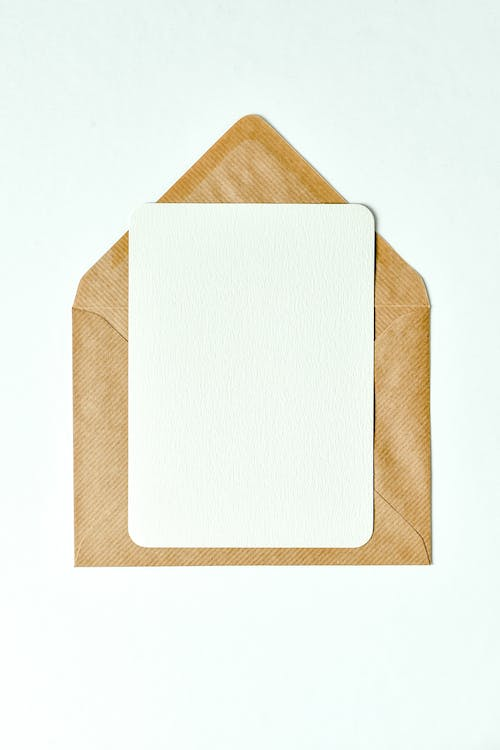
\includegraphics[width=\textwidth]{media/image8.jpeg}
%\end{figure}

\num{1} O que são cartas pessoais?

\reduline{Cartas pessoais são correspondências trocadas entre pessoas.\hfill}
\linhas{2}

\num{2} Quem escreveu a carta?

\reduline{O autor da carta é Guilherme\hfill}
\linhas{1}

\num{3} Quem recebeu a carta?

\reduline{O destinatário da carta é o pai do Guilherme\hfill}
\linhas{1}

\num{4} De onde Guilherme escreveu a carta?

\reduline{Guilherme escreveu a carta de Fortaleza\hfill}
\linhas{1}

\num{5} Como é composta a saudação da carta lida e o que ela indica sobre a
relação entre remetente e destinatário?

\reduline{``Olá, amado papai!'' é a saudação que indica que Guilherme,
o remetente, é filho do destinatário e o trata com afetividade.\hfill}
\linhas{2}

\num{6} Qual é o assunto da carta?

\reduline{Na carta a seu pai, Guilherme conta que está
bem, comenta o que mais gostou em Fortaleza, diz quando pretende voltar
para casa e fala sobre a saudade que está sentindo dos familiares e
amigos de infância.\hfill}
\linhas{2}

\num{7} A carta pessoal apresentada tem uma linguagem formal ou informal?
Justifique sua resposta.

\reduline{A carta pessoal normalmente é escrita de modo informal, 
tendo em vista que é uma correspondência entre pessoas íntimas,
com demonstração de afetividade e carinho. Na carta de Guilherme a seu
pai, a informalidade fica evidente pela utilização de termos como ``amado 
papai'' e frases como ``sinto falta de vocês'', cujo conteúdo é indicador
de afetividade, além de formas verbais flexionadas na primeira pessoa, 
por meio das quais o remetente fala de suas impressões pessoais.\hfill}
\linhas{2}

%A questão abaixo foi suprimida, porque não faz sentido no contexto
%\num{8} O texto apresentado é teatral. Com qual objetivo esses textos são
%escritos?

%\reduline{O objetivo de se escrever textos desse tipo é para que sejam encenados.\hfill}
%\linhas{2}

\num{8} Leia a carta a seguir e responda às questões propostas.

\begin{mdframed}[linewidth=10pt,linecolor=salmao!20,backgroundcolor=salmao!20,roundcorner=20pt]
\begin{flushright}
Curitiba, 12 de fevereiro de 2023.
\end{flushright}

\emph{Querida filha Cecília},

Estou morrendo de saudades...

Por aqui, a vida está exatamente igual, seus irmãos e seu pai também
estão bem, e sentem muitas saudades de você.

Filhinha, você está fazendo o certo. Ir a São Paulo estudar vai te
ajudar muito a conseguir o emprego dos seus sonhos.

Aproveite muito filha, ajude a sua prima Sofia com as tarefas domésticas
e agradeça sempre por ela ter recebido você na casa dela.

\begin{flushright}
Beijo,

Mamãe.
\end{flushright}
\end{mdframed}

\begin{escolha}
\item \textbf{Vocativo} é o modo como é denominado quando chamamos uma
pessoa com quem estamos nos comunicando. Sublinhe o vocativo da carta
acima.

\item Quem escreveu a carta?

\begin{boxlist}
\boxitem{X} a mãe de Cecília 

\boxitem{\white{X}} Sofia

\boxitem{\white{X}} Cecília
\end{boxlist}

\item Quem é Cecília com relação a pessoa que escreve a carta??

\reduline{Filha.\hfill}
\linhas{1}

\item Quem é o destinatário dessa carta?

\reduline{Cecília.\hfill}
\linhas{1}

\item Escreva qual foi a despedida da carta. 

\reduline{Beijo, Mamãe.\hfill}
\linhas{1}
\end{escolha}

\colorsec{Treino}

\num{1} Leia a carta pessoal a seguir para responder à questão.

%(Fácil) 

\begin{mdframed}[linewidth=10pt,linecolor=salmao!20,backgroundcolor=salmao!20,roundcorner=20pt]
\begin{flushright}
São Paulo, 01 de março de 2023.
\end{flushright}

Querida vó,

Como a senhora está? Estou com muitas saudades de você e mal posso
esperar pelo Natal, quando vamos nos reunir e relembrar os tempos de
infância. Estar longe de você tem sido muito triste, mas guardo os seus
conselhos que me ajudam a superar as dificuldades.

\begin{flushright}
Até breve!

Sandra
\end{flushright}
\end{mdframed}

O elemento ``Até breve,'' da carta lida, representa a:

\begin{multicols}{2}
\begin{escolha}
\item assinatura.

\item despedida.

\item saudação.

\item reclamação.
\end{escolha}
\end{multicols}

\num{2} Releia a carta pessoal a seguir para responder à questão.

%(Médio) 

\begin{mdframed}[linewidth=10pt,linecolor=salmao!20,backgroundcolor=salmao!20,roundcorner=20pt]
\begin{flushright}
São Paulo, 01 de março de 2023.
\end{flushright}

Querida vovó,

Como a senhora está? Estou com muitas saudades de você e mal posso
esperar pelo Natal, quando vamos nos reunir e relembrar os tempos de
infância. Estar longe de você tem sido muito triste, mas guardo os seus
conselhos que me ajudam a superar as dificuldades.

\begin{flushright}
Até breve!

Sandra
\end{flushright}
\end{mdframed}

\pagebreak
Que saudação seria mais adequada ao contexto dessa carta?

\begin{multicols}{2}
\begin{escolha}
\item Prezada avó.

\item Olá, vovó!

\item Avó.

\item Atenciosamente.
\end{escolha}
\end{multicols}



\num{3} Leia a carta de uma leitora para a revista de publicações
científicas denominada \textit{Planeta}.

%(Difícil) 

\begin{quote}
\textbf{Evolução com consciência}

Sou leitora e apreciadora assídua de PLANETA. Quero parabenizar Ricardo
Arnt por estar assumindo a direção de redação. Aproveito para desejar a
toda a equipe da revista um tempo de muita paz e luz. Tenho acompanhado
muitas mudanças, algumas muito positivas e outras, a meu ver, não tão
positivas sobre a filosofia da revista, mas mudanças não podem agradar a
todos. O importante é que continue a ser uma publicação que nos ajude em
nosso evoluir com consciência, mesmo que por trilhas diferenciadas das
antigas.

\begin{flushright}
Almira Lima, Rio Grande, RS, por \emph{e-mail}.
\end{flushright}

\fonte{Almira Lima. Revista Planeta. Evolução com consciência.
Disponível em: www.revistaplaneta.com.br/cartas-15/. Acesso em: 24 Abr. 2023.}
\end{quote}

\begin{tabular}{ll}
\textbf{Glossário} & \mbox{}\\
assídua & com bastante frequência.\\
\end{tabular}

Sobre a carta acima, é correto afirmar que 

\begin{escolha}
\item o remetente da carta é ``Planeta''.

\item ``muita paz e luz'' é a despedida.

\item o título é ``sou leitora e apreciadora''.

\item ``Rio Grande'' é a localização da leitora.
\end{escolha}



\chapter{Textos instrucionais}
\markboth{Módulo 3}{}

%\coment{Neste módulo, o objetivo é habilitar os alunos a reconhecer textos instrucionais e suas características.}
\vspace*{-1cm}\enlargethispage{\baselineskip}

\colorsec{Habilidades do SAEB}

\begin{itemize}
\item Analisar elementos constitutivos de gêneros textuais diversos.

\item Reconhecer os usos da pontuação.

\item Analisar os efeitos de sentido decorrentes do uso da pontuação.
\end{itemize}

\colorsec{Habilidade da BNCC}

\begin{itemize}
	\item 
EF04LP13.
\end{itemize}

\conteudo{
\textbf{Textos instrucionais}

\begin{wrapfigure}{l}{.5\textwidth}

\includegraphics[width=.5\textwidth]{media/image9.png}
\end{wrapfigure}

No nosso dia a dia, em diversas situações, precisamos ler textos que nos
ajudem a executar uma tarefa. Quando queremos fazer um bolo, por
exemplo, procuramos uma \textbf{receita}. Lemos um \textbf{manual} quando
queremos saber quais são as regras de um jogo, ou a \textbf{bula} quando
queremos compreender como tomar determinada medicação. Todos esses textos
que nos ensinam o que fazer para atingir um objetivo são
denominados \textbf{instrucionais}, porque fornecem instruções.

O objetivo dos textos instrucionais é informar como devemos
proceder para realizar uma tarefa. Eles devem ser simples, objetivos,
diretos e esclarecedores e são repletos de verbos, como
``precisar'', ``necessitar'' e ``dever'' para informar ao leitor os
procedimentos a cumprir.
}

\colorsec{Atividades}

\num{1} Leia o texto a seguir. Em seguida, responda às atividades propostas.


\begin{figure}[htpb!]
\centering
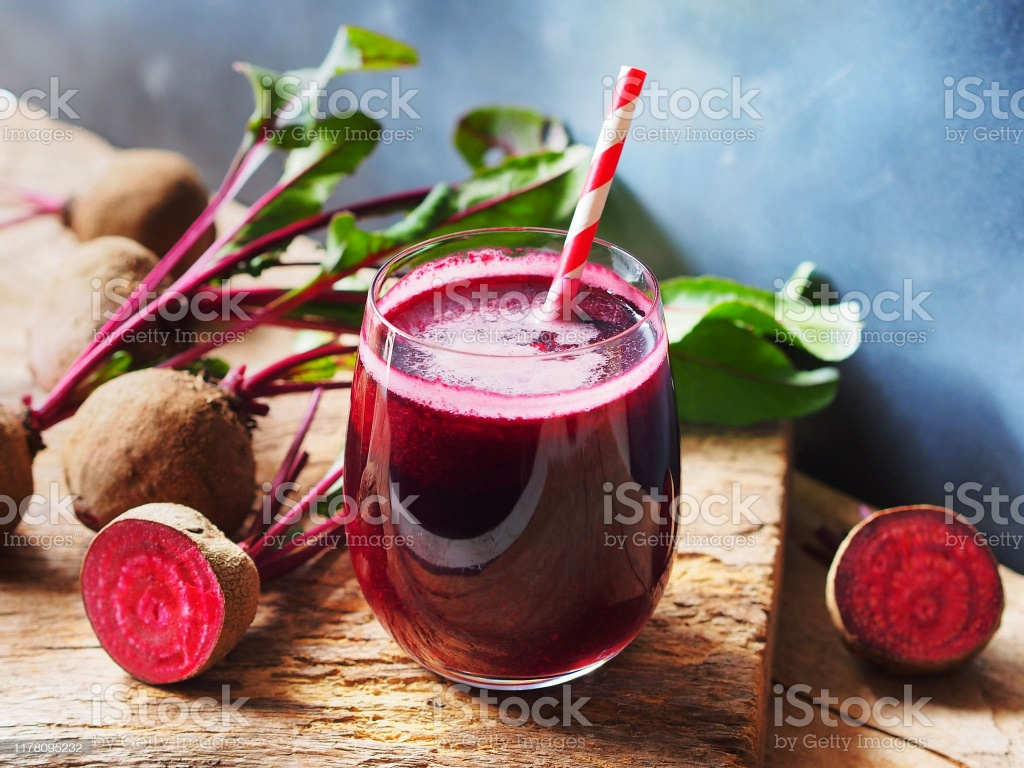
\includegraphics[width=.7\textwidth]{media/image10.jpeg}
\end{figure}

\begin{quote}
\textbf{Suco de beterraba com limão}

\textbf{Ingredientes}

2 copos americanos duplos de água

1 beterraba média

1 limão sem casca e sementes

1 colher de sopa de açúcar

\textbf{Modo de preparo}

Misture tudo no liquidificador. Se desejar, coloque gelo e sirva.

\textbf{Rendimento}

3 porções.

Dica: O limão pode ser substituído por laranja ou maracujá.

\fonte{Ministério da Saúde. Suco rico em fibras: 5 receitas para misturar frutas e vegetais. Disponível em:
https://www.gov.br/saude/pt-br/assuntos/saude-brasil/eu-quero-me-alimentar-melhor/noticias/2018/suco-rico-em-fibras-5-receitas-para-misturar-frutas-e-vegetais/.
Acesso em: 24 abr. 2023.}
\end{quote}

\begin{escolha}
\item Por que podemos dizer que o texto lido é do tipo instrucional?

\reduline{O texto lido pode ser considerado instrucional porque é uma receita de
suco, ou seja, propõe-se a ensinar como prepará-lo. Para isso, dá
instruções do que deve ser feito pelo leitor, quais são os ingredientes
necessários e o modo de preparo.\hfill}
\linhas{3}

\item Qual é a quantidade de beterraba e de açúcar que devem ser utilizadas
para fazer o suco?

\reduline{Para fazer o suco, é necessário usar 1 beterraba média e 1
colher de açúcar.\hfill}
\linhas{1}

\item Como você descobriu essa informação?

\reduline{A informação está presente na lista de ingredientes da receita.\hfill}
\linhas{1}

\item No modo de preparo, por que não é necessário expor a quantidade de
ingredientes que devem ser utilizadas?

\reduline{A quantidade já foi informada na lista de ingredientes\hfill}
\linhas{1}
\end{escolha}

\pagebreak
\num{2} Releia este trecho da receita atentando aos verbos destacados:

\begin{quote}
\textbf{Misture} tudo no liquidificador. Se desejar, \textbf{coloque} gelo e sirva.
\end{quote}

\begin{escolha}
\item
  Os verbos destacados foram utilizados no texto para:

\begin{boxlist}
\boxitem{\white{X}} mostrar quem faz a ação.

\boxitem{X} fazer pedidos.

\boxitem{\white{X}} dar instruções.

\boxitem{\white{X}} indicar o tempo em que a ação acontece.
\end{boxlist}

\item
  Os verbos destacados estão no modo:

\begin{boxlist}
\boxitem{X} imperativo

\boxitem{\white{X}} afirmativo
\end{boxlist}

\end{escolha}

\num{3} Leia o passo a passo de como fazer um coração de origami.

%Arte: Pedir autorização do texto e imagem a seguir ou solicitar ilustração conforme modelo a seguir.
\begin{figure}[htpb!]
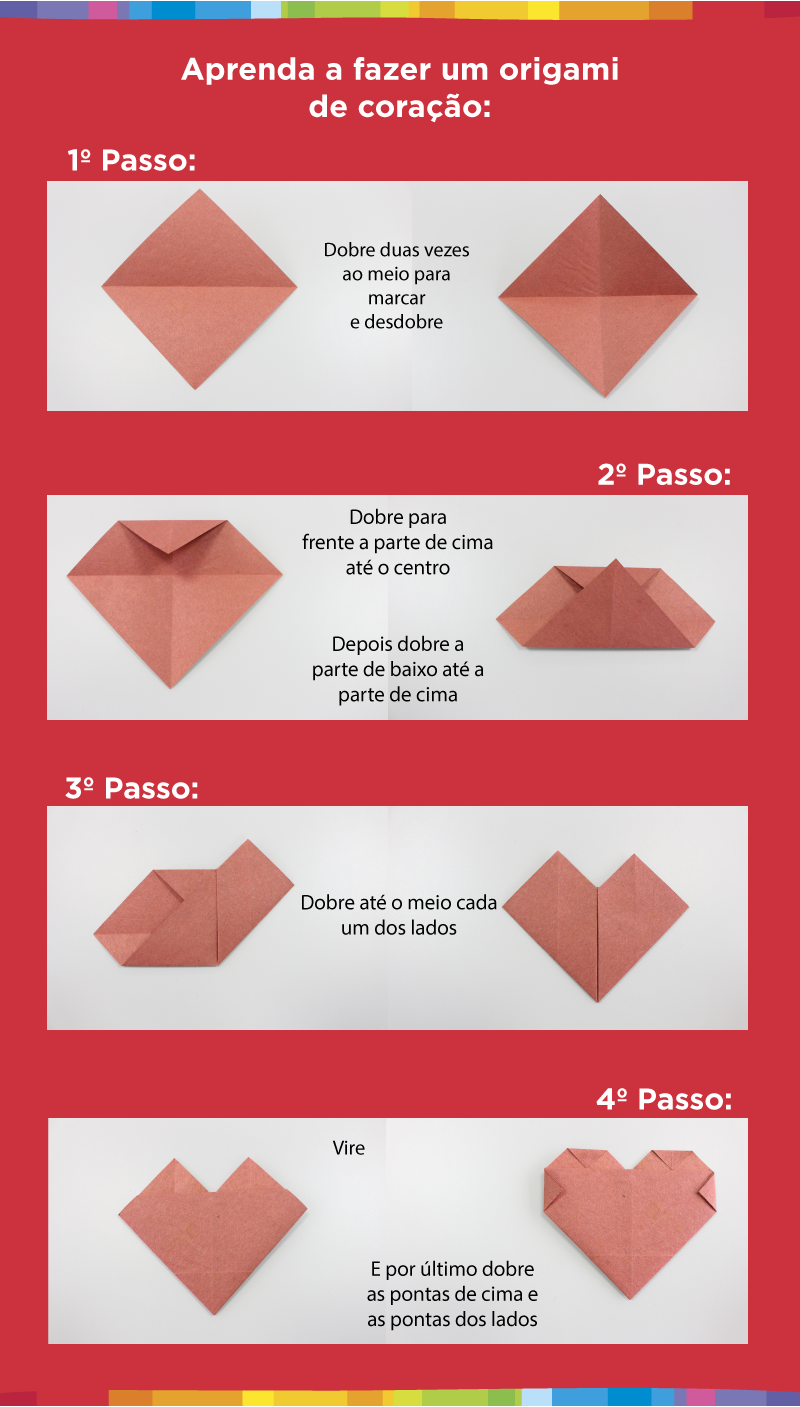
\includegraphics[width=\textwidth]{media/image11.png}
\end{figure}

%Disponível em: https://blog.brandili.com.br/diy-como-fazer-um-origami-de-coracao/. Acesso em: 6 mar. 2023.

\begin{escolha}
\item Por que o texto lido pode ser considerado um texto instrucional? Justifique sua resposta.

\reduline{O texto pode ser considerado instrucional porque sua finalidade
é auxiliar o leitor a realizar determinada tarefa, por meio de instruções
específicas.\hfill}

\item Qual é o objetivo do texto lido?

\reduline{O objetivo do texto lido é ensinar a fazer um origami em forma de coração.\hfill}

\item Que características do texto instrucional podem ser encontradas no texto lido?

\reduline{O título em destaque, apresentando claramente o que o leitor
vai aprender a fazer; a organização em quatro passos distintos, bem 
separados visualmente; as formas verbais no imperativo; as imagens 
explicativas --- todas essas características permitem afirmar que o 
texto em destaque é instrucional.\hfill}
\end{escolha}

\colorsec{Treino}

\num{1} Leia o texto a seguir.

%(Fácil)
\begin{quote}
\begin{wrapfigure}{r}{.5\textwidth}
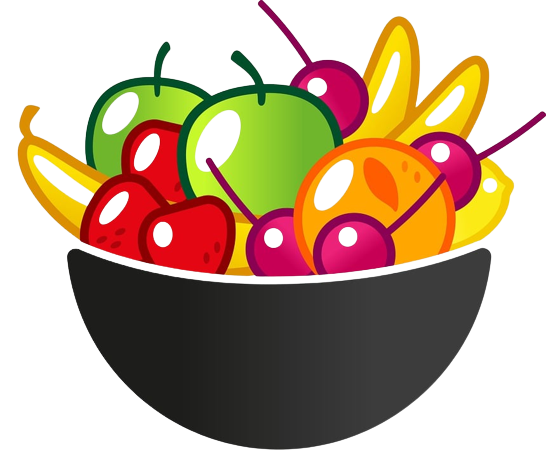
\includegraphics[width=.5\textwidth]{media/image12.png}
\end{wrapfigure}

\textbf{Salada de frutas}

\textbf{Ingredientes:}

\begin{itemize}
\item 1 maçã

\item 3 bananas

\item ½ mamão

\item 1 lata de leite condensado (opcional) ou açúcar.
\end{itemize}

\textbf{Modo de preparo:}

Lave bem todas as frutas. Retire a casca e as sementes. Corte as frutas
e quadradinhos. Coloque o leite condensado ou o açúcar. Misture e leve à
geladeira por 30 minutos.
\end{quote}

\pagebreak
O texto lido pode ser classificado como:

\begin{escolha}
\item
  receita culinária.
\item
  reportagem.
\item
  instrução de jogos.
\item
  fábula.
\end{escolha}

\num{2} Leia o texto instrucional a seguir.

%(Médio)

\begin{quote}
\textbf{Quem toca mais, ganha}

\textbf{Material necessário}\\
1 bola

\textbf{Modo de jogar}\\
Em um campo aberto, duas equipes têm como
objetivo trocar o maior número possível de passes.

Cada toque representa um número na contagem, que deve ser feita
paralelamente aos passes, em voz alta.

Quando um passe sofrer interferência da equipe adversária, a contagem
recomeça do zero.

\fonte{Ana Rosa Abreu e outros autores. Quem toca mais, ganha. Alfabetização: livro
do aluno, Vol.3: textos informativos, textos instrucionais e biografias.
Disponível em: www.dominiopublico.gov.br/download/texto/me000590.pdf. 
Acesso em: 24 abr. 2023. com alterações}
\end{quote}

Em relação à estrutura do texto instrucional, pode-se identificar a
presença de subtítulos que

\begin{escolha}
\item mostram como obter o material e escolher os participantes.

\item explicam o funcionamento do material ``bola''.

\item listam o objeto necessário e a maneira de jogar.

\item apresentam diferentes modos de jogar o jogo.
\end{escolha}

\pagebreak
\num{3} Leia o trecho de um manual.
%(Difícil) 

\begin{quote}
UNO® é recomendado para crianças e adultos a partir de 7 anos de idade e número de jogadores pode variar entre 2 e 10 pessoas.

\textbf{Baralho}\\
Para jogar UNO® é necessário comprar um baralho próprio para o jogo. Esse baralho é composto por 108 cartas.

\textbf{Objetivo}\\
Ser o primeiro jogador a fazer 500 pontos. Para fazer pontos, você deve
livrar-se o quanto antes de todas as cartas da sua mão e usar as cartas 
de ação para evitar que os adversários façam o mesmo. A quantidade de 
pontos que você ganha é a soma dos números das cartas dos oponentes.

\fonte{Alfabetizando e Letrando. Texto Instrucional: Jogo UNO®. Disponível em: http://nancinaliniprof.blogspot.com/2020/05/texto-instrucional-jogo-uno.html
Acesso em: 24 abr. 2023. com alterações.}
\end{quote}
%Aqui um problema: o link apresentado pelo autor não levava a lugar nenhum. Encontrei o tal manual de jogo nesse blog de uma professora. Me digam se dá para usar.  

Conforme informações do texto, para ganhar o jogo a pessoa deve

\begin{escolha}
\item ser a primeira a fazer 500 pontos.

\item possuir pelo menos uma carta nas mãos.

\item evitar usar as cartas de ação durante o jogo.

\item ter menos pontos que as cartas dos oponentes.
\end{escolha}

\chapter{Anúncio Publicitário}
\markboth{Módulo 4}{}

%\coment{Neste módulo, espera-se que os alunos leiam e compreendam autonomamente textos do campo da vida pública; relacionem a imagem no texto à mensagem escrita (linguagens verbal e não verbal); relacionem a finalidade do texto às estratégias de convencimento; identifiquem a função social do texto, reconhecendo para que serve e a quem se destina; identifiquem a ideia central do texto, compreendendo-o globalmente e infiram informações implícitas no texto.}

\colorsec{Habilidades do SAEB}

\begin{itemize}
\item Analisar o uso de recursos de persuasão em textos verbais e/ou multimodais.

\item Analisar os efeitos de sentido de recursos multissemióticos em textos que circulam em diferentes suportes.

\item Julgar a eficácia de argumentos em textos.
\end{itemize}

\colorsec{Habilidades da BNCC}

\begin{itemize}
	\item 
EF03LP19
\end{itemize}

\conteudo{
\textbf{Anúncio publicitário}\bigskip

%\textbf{https://pixabay.com/pt/photos/cartazes-muro-propaganda-679177/}
\noindent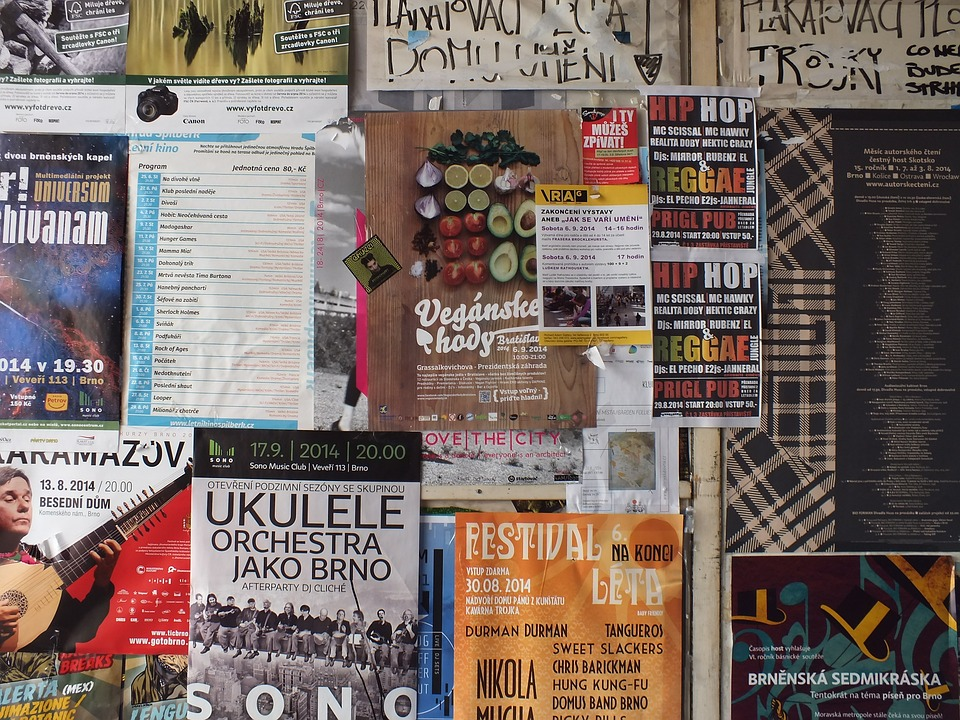
\includegraphics[width=\textwidth]{media/image13.jpeg}

O \textbf{anúncio publicitário} é um texto com a finalidade de
convencer o leitor a consumir um produto ou serviço. Para esse objetivo,
utiliza linguagem persuasiva, misturando recursos visuais, como cores,
formas, símbolos, figuras, imagens fictícias, entre outros, com uma
linguagem cheia de afeto, emoções com a intenção de envolver o
consumidor em um jogo linguístico, despertar o interesse e provocar
vontades que o levem a comprar o produto ou o serviço.

A \textbf{campanha publicitária} é o conjunto de peças publicitárias,
criado por uma agência, a fim de divulgar um produto ou
determinada ideia.
}

\colorsec{Atividades}

\num{1} O dia 20 de novembro foi oficialmente incluído no calendário 
nacional como data de celebração da memória de Zumbi dos Palmares e da
consciência negra. Leia o cartaz publicitário a seguir.

%\coment{Explore com os alunos o cartaz, a imagem que o compõe e os elementos verbais. Avalie com eles os motivos da escolha do produtor ao dar ênfase a alguns elementos do texto verbal e se esse recurso foi efetivo na divulgação do que pretendia.}

%https://www.guiricema.mg.gov.br/20-de-novembro-dia-da-consciencia-negra/
\begin{figure}[htpb!]
\centering
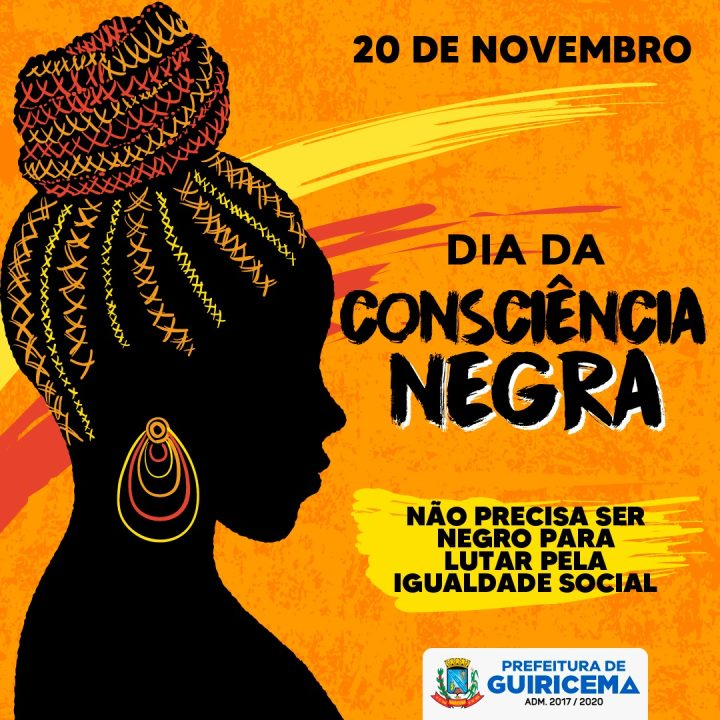
\includegraphics[width=.6\textwidth]{media/image14.jpeg}
\end{figure}

\pagebreak

\begin{escolha}
\item O cartaz da campanha do \textbf{Dia da Consciência Negra} foi feito para:

\begin{boxlist}
\boxitem{X} convencer as pessoas em relação à importância de lutar pela igualdade racial.

\boxitem{\white{X}} convencer as pessoas em relação à importância de todos terem acesso à vacinação.

\boxitem{\white{X}} sensibilizar as pessoas, como ocorre nas poesias.
\end{boxlist}

\item Releia o \emph{slogan} do cartaz.

\begin{mdframed}[linewidth=10pt,linecolor=salmao!20,backgroundcolor=salmao!20,roundcorner=20pt]
\textbf{Não precisa ser negro para lutar pela igualdade racial}
\end{mdframed}

Que sentido pode ter essa frase? Converse com os colegas e escreva a
conclusão a que chegaram nas linhas a seguir.

\reduline{Resposta pessoal. Explique aos alunos que, embora no Brasil haja
uma intensa mistura de raças, a incidência de racismo pode não ser tão
evidente para determinadas pessoas, mas ele não deixa de existir. Em alguns
casos, ele ocorre de forma sutil e não é percebido pelas pessoas. É
necessário fortalecer a identidade étnico-racial e respeitar as
diversidades.\hfill}

\item Quem promoveu esse cartaz?

\reduline{A Prefeitura de Guiricema promoveu o cartaz analisado.\hfill}
\linhas{1}

\item Em sua opinião, o anúncio está cumprindo seu propósito? Justifique 
sua resposta.

\reduline{Resposta pessoal.\hfill}
\linhas{1}
\end{escolha}

\num{2} Leia, a seguir, o cartaz de promoção do Festival Nacional do Teatro
Infantil, de Feira de Santana, Bahia.

%https://jornalgrandebahia.com.br/2017/09/a-festa-do-teatro-infantil-brasileiro-vai-comecar-em-feira-de-santana/
\begin{figure}[htpb!]
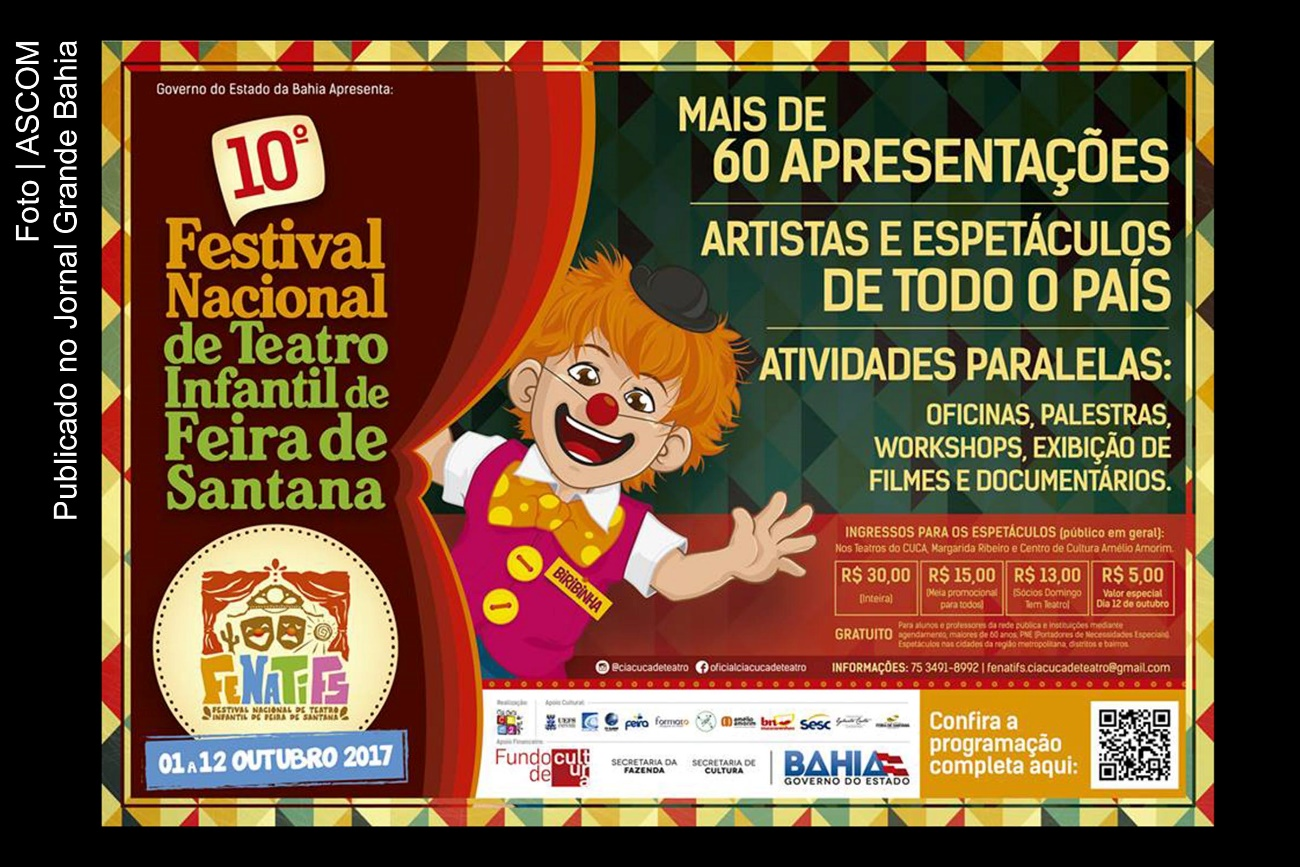
\includegraphics[width=\textwidth]{media/image15.jpeg}
\end{figure}

\begin{escolha}
\item Quais estratégias, na composição dessa capa, contribuem para
incentivar as pessoas a participar do festival?

\reduline{Os alunos podem citar o colorido do cartaz, a ilustração de uma
criança com nariz de palhaço e roupa de bilheteiro, a quantidade atrações 
no festival e as atividades paralelas que serão realizadas durante o evento.\hfill}

\item Quantas vezes ocorreu o Festival Nacional de Teatro Infantil de
Feira de Santana?

\reduline{O Festival Nacional de Teatro Infantil de Feira de Santana já aconteceu 10 vezes\hfill}

\item Quais são as atividades paralelas que vão ocorrer durante o festival?

\reduline{Oficinas, palestras, \emph{Workshops}, exibição de filmes e documentários.\hfill}

\item As cores e letras usadas no cartaz foram utilizadas com o objetivo de:

\begin{boxlist}
\boxitem{\white{X}} deixá-lo mais bonito.

\boxitem{X} destacar a mensagem escrita.

\boxitem{\white{X}} destacar um produto
\end{boxlist}

\item Por que foi usado um desenho de um personagem infantil no cartaz?

\reduline{O desenho de um personagem infantil foi usado para atrair a atenção das crianças.\hfill}
\linhas{1}

\item Quando esse festival aconteceu? 

\reduline{O festival ocorreu de 01 a 12 de outubro de 2017.\hfill}
\linhas{1}
\end{escolha}

\num{3} Você sabe o que é um \textbf{festival}? Junte-se a um colega,
pesquisem no dicionário o significado dessa palavra e registrem a seguir 
o que vocês encontraram.

\reduline{Festivais são eventos ou espetáculos 
culturais que ocorrem periodicamente, com diversas apresentações.\hfill}
\linhas{5}

\pagebreak
\num{4} Leia, agora, outro anúncio de campanha publicitária.

%https://www.facebook.com/daejundiai/photos/a.609606715910778/1544172665787507/?type=3
\begin{figure}[htpb!]
\centering
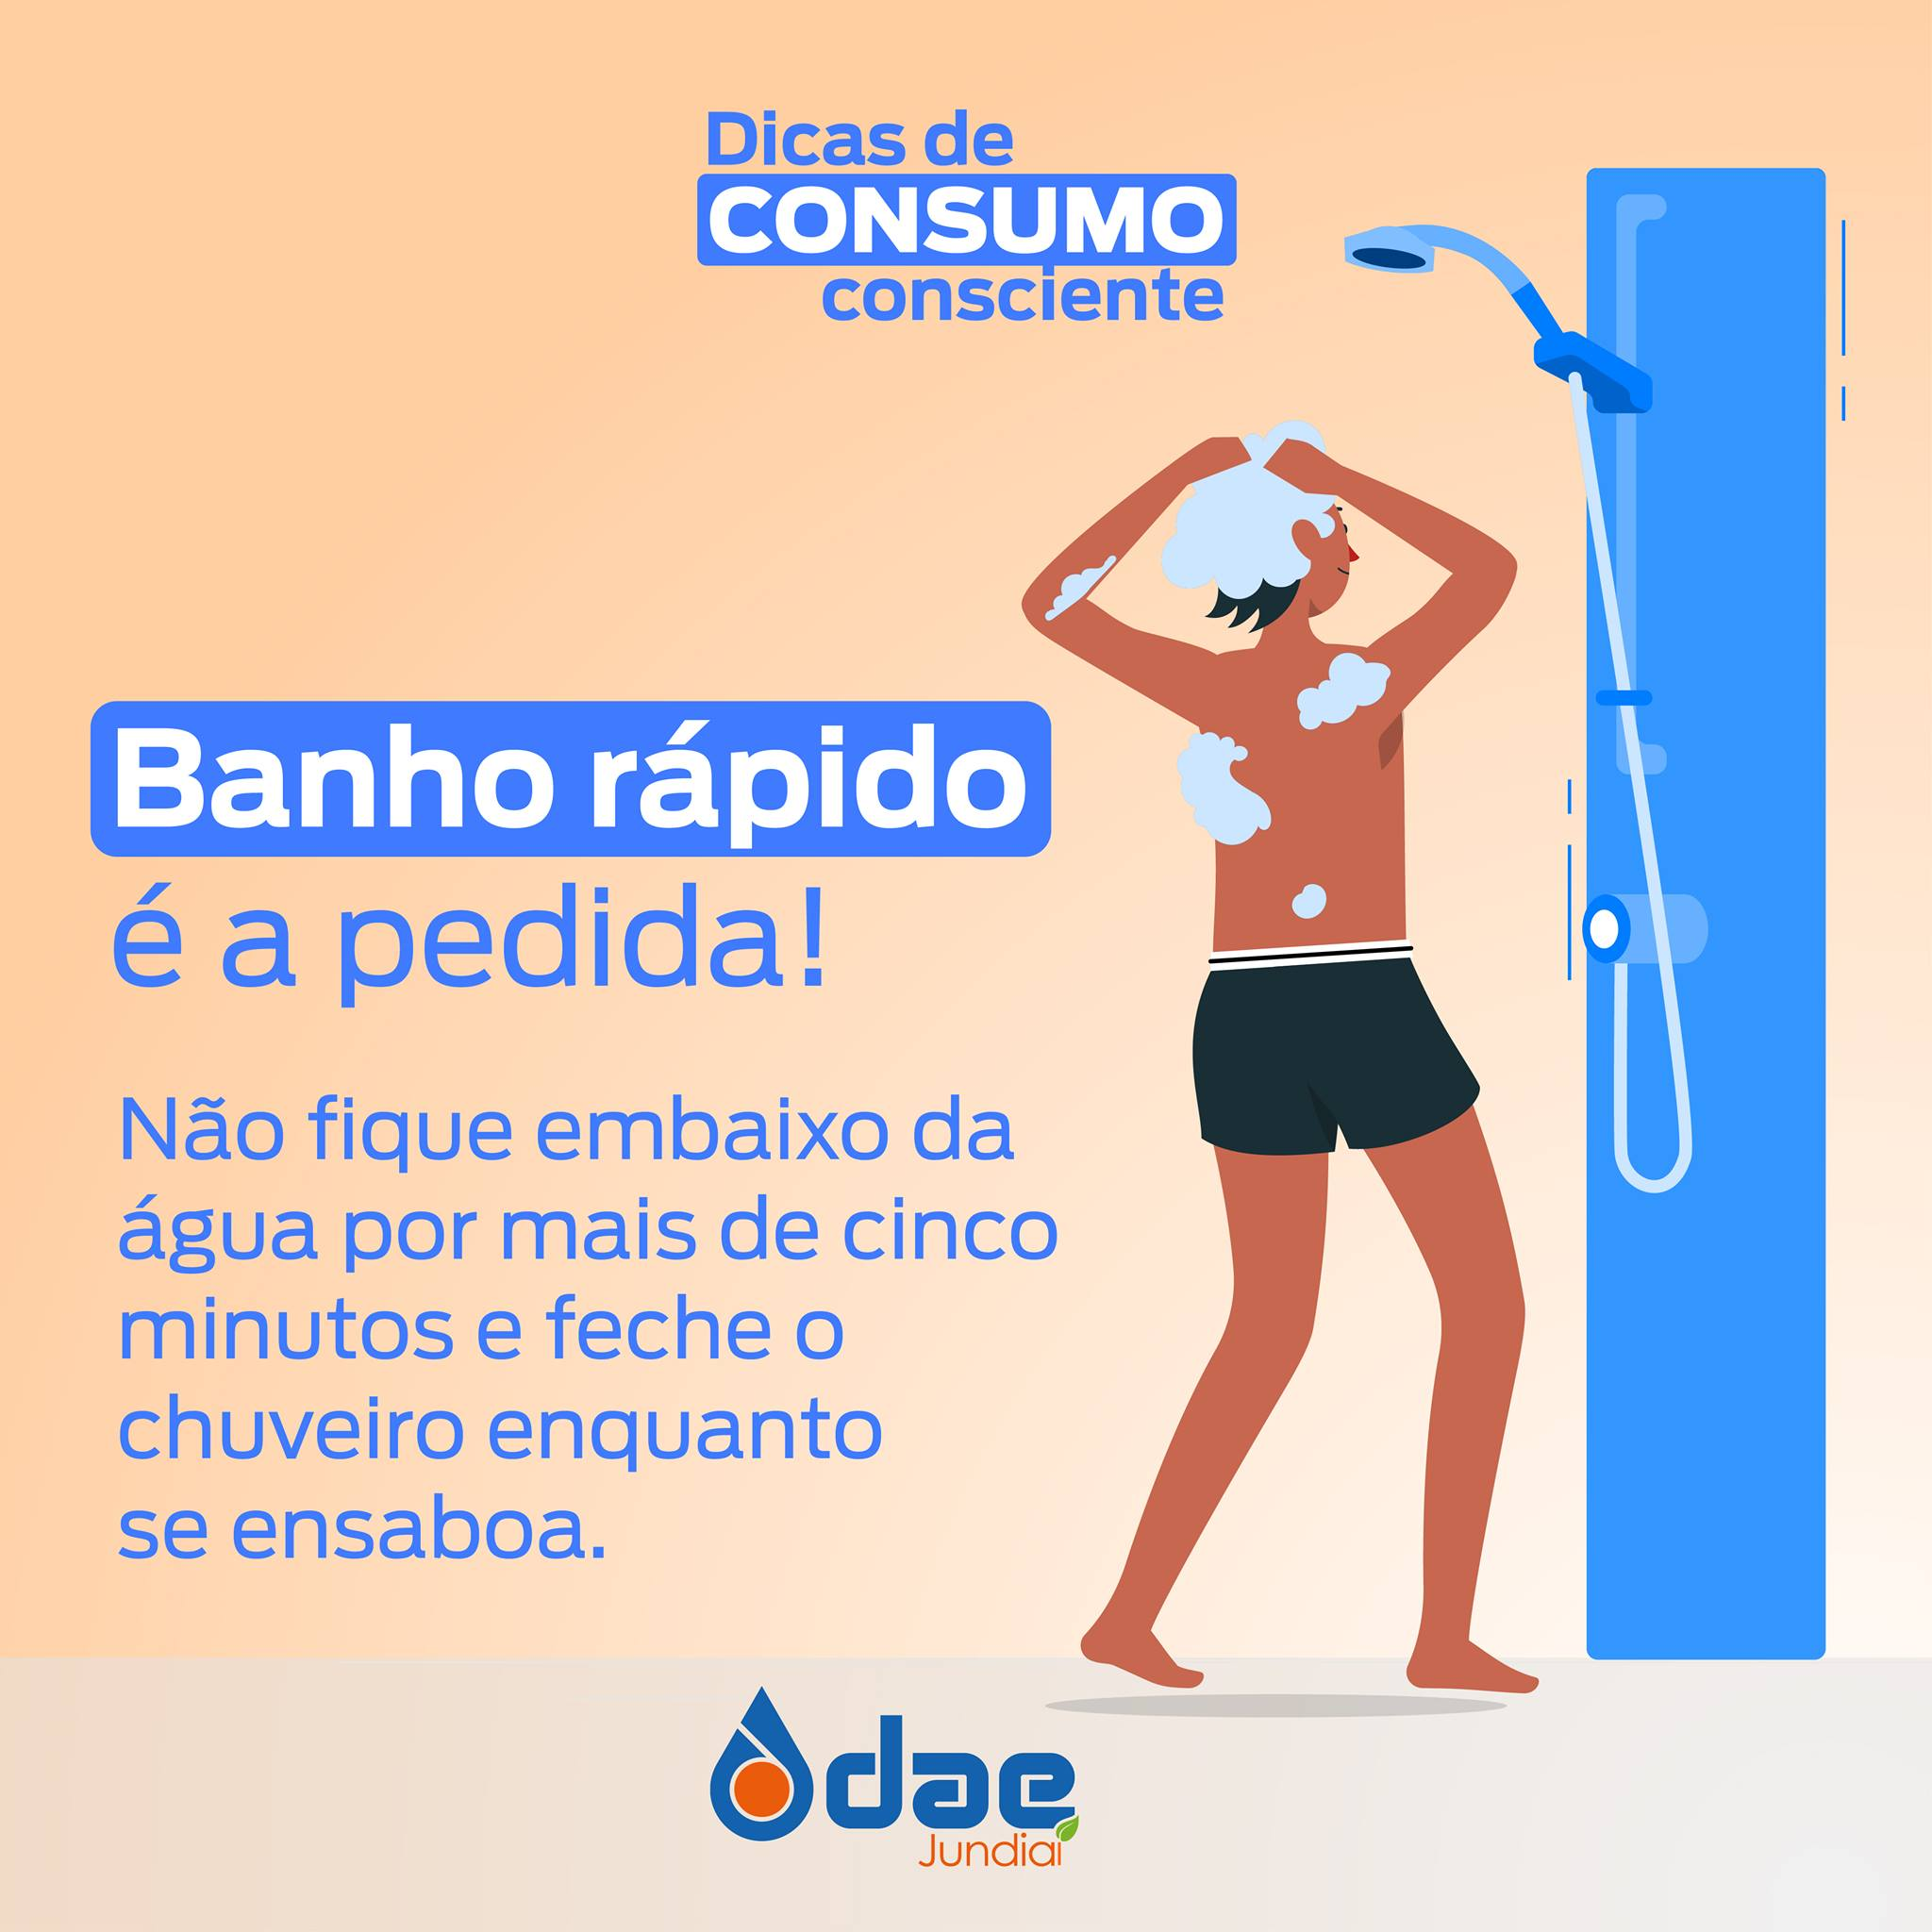
\includegraphics[width=.7\textwidth]{media/image16.jpeg}
\end{figure}

\begin{escolha}
\item Qual é o objetivo dessa campanha?

\reduline{O objetivo da campanha é a conscientização a respeito da economia
de água durante o banho.\hfill}
\linhas{2}

\item Segundo o cartaz, como se pode economizar água durante o banho?

\reduline{Para economizar água, o banho não deve durar mais de cinco minutos
e o chuveiro deve ser fechado enquanto se ensaboa.\hfill}
\linhas{1}

\item O objetivo desse cartaz é convencer os leitores a repensar ou mudar
de atitude. Você foi convencido? Justifique sua resposta.

\reduline{Resposta pessoal. Aproveite o momento e explique aos alunos que a
economia de água não apenas preserva o ambiente, mas também implica
economia financeira, tendo em vista que a conta diminui. Vale lembrar,
ainda, que a água que chega à nossa casa tem custos de captação,
tratamento e distribuição.\hfill}
\end{escolha}

\colorsec{Treino}

\num{1} Leia o cartaz relacionado à água.
%(Fácil)
%https://www.saopedro.sp.gov.br/saaesp-faz-atividade-especial-para-celebrar-dia-mundial-da-agua
\begin{figure}[htpb!]
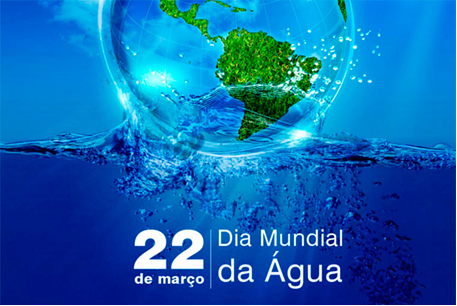
\includegraphics[width=\textwidth]{media/image17.png}
\end{figure}

%Paulo: colocar aqui a imagem do link a seguir. 

\fonte{Prefeitura de Ipê. O Dia Mundial da Água. Disponível em:
https://www.pmipe.rs.gov.br/noticias/o-dia-mundial-da-agua.
Acesso em: 25 abr. 2023.}

%Fábia e Felipe: o link sugerido pelo autor foi tirado do ar. Além disso, na minha opinião, a questão não era adequada. A imagem não permite afirmar que a finalidade do cartaz é ``conscientizar sobre o uso de forma econômica e sem desperdícios''. A alternativa correta força uma inferência que extrapola o cartaz. Tentei melhorar, mas ainda não dei por satisfeito.    

\pagebreak
Relacionando a imagem do cartaz com as frases nele apresentadas, podemos
afirmar que 

\begin{escolha}
\item a qualidade de vida do homem não depende da água.

\item o uso adequado da água permite qualidade de vida.

\item a água é um recurso natural ilimitado da humanidade.

\item a escassez da água já foi solucionada pela ciência.
\end{escolha}


\num{2} Analise a campanha de doação de sangue.

%http://www.moreirasales.pr.gov.br/noticia/2203/doe-sangue-salve-vidas-campanha-de-doacao-de-sangue-sera-realizado-na-proxima-semana/
\begin{figure}[htpb!]
\centering
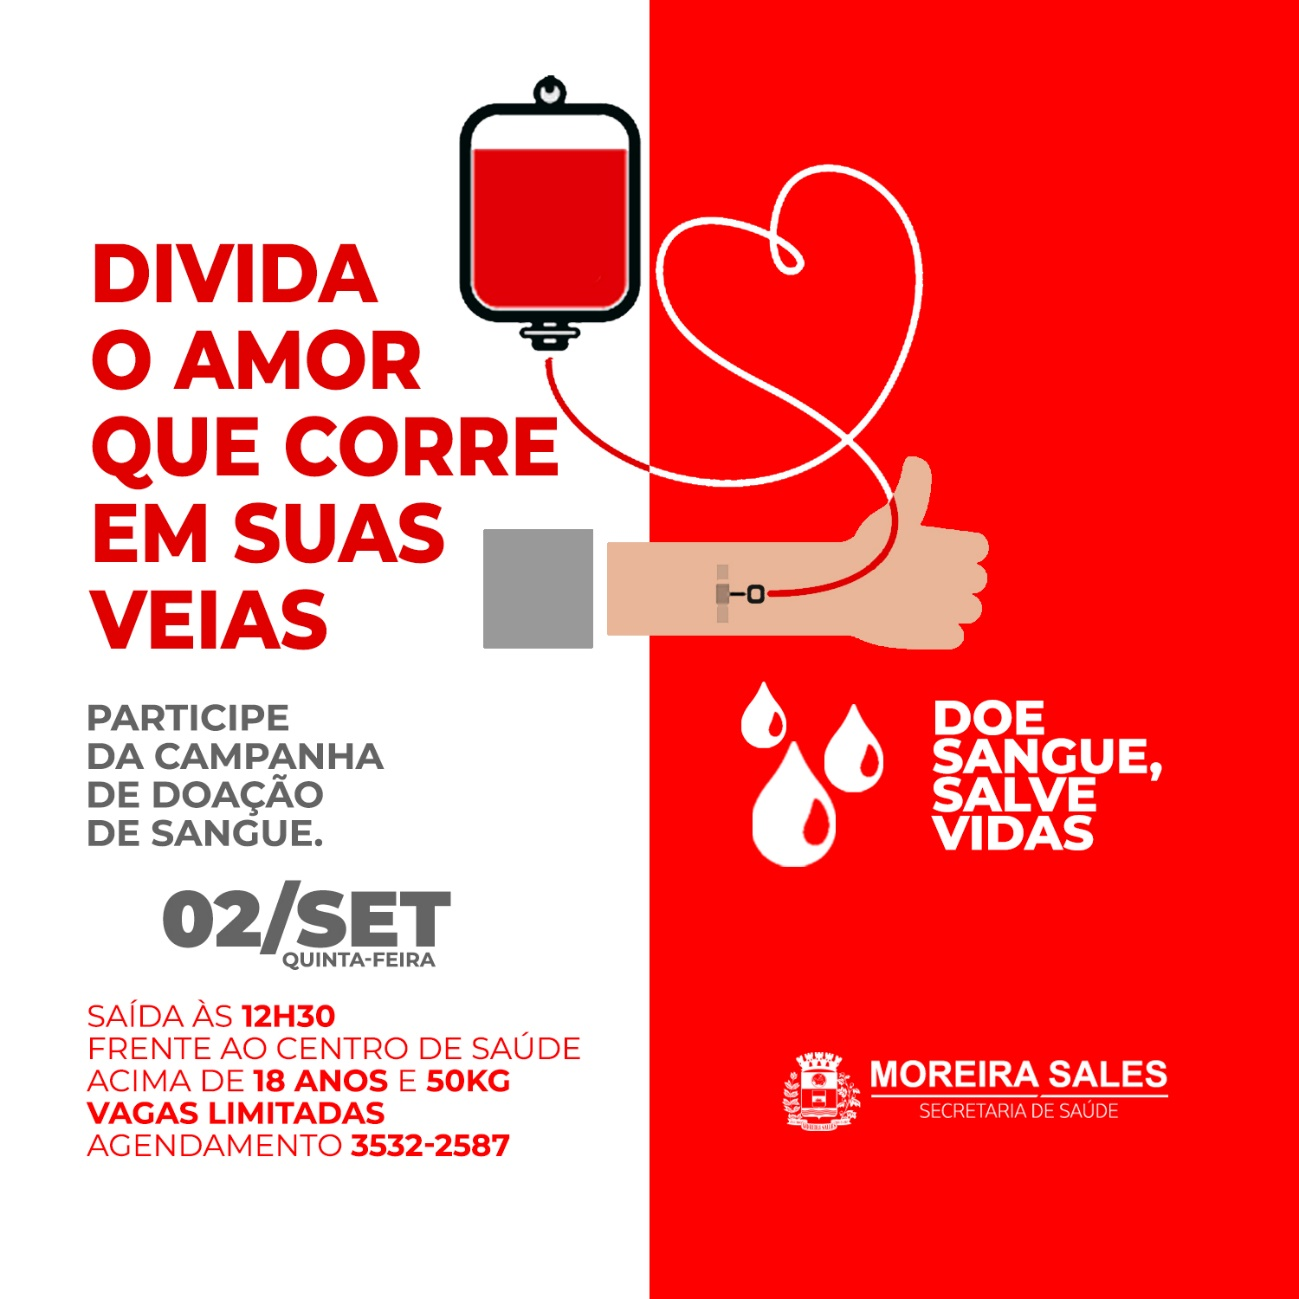
\includegraphics[width=.6\textwidth]{media/image18.jpeg}
\end{figure}
%Disponível em: \url{http://www.moreirasales.pr.gov.br/noticia/2203/doe-sangue-salve-vidas-campanha-de-doacao-de-sangue-sera-realizado-na-proxima-semana/}. Acesso em: 7 mar. 2023.

O \emph{slogan} da campanha é

\begin{escolha}
\item ``doe sangue, salve vidas''.

\item ``divida o amor que corre nas suas veias''.

\item ``participe da campanha de doação de sangue''.

\item ``Moreira Sales''.
\end{escolha}

\pagebreak
\num{3} Leia o cartaz a seguir, observando as imagens e o texto. 

%(Difícil)

%www.saude.pr.gov.br/modules/noticias/article.php?storyid=4950
\begin{figure}[htpb!]
\centering
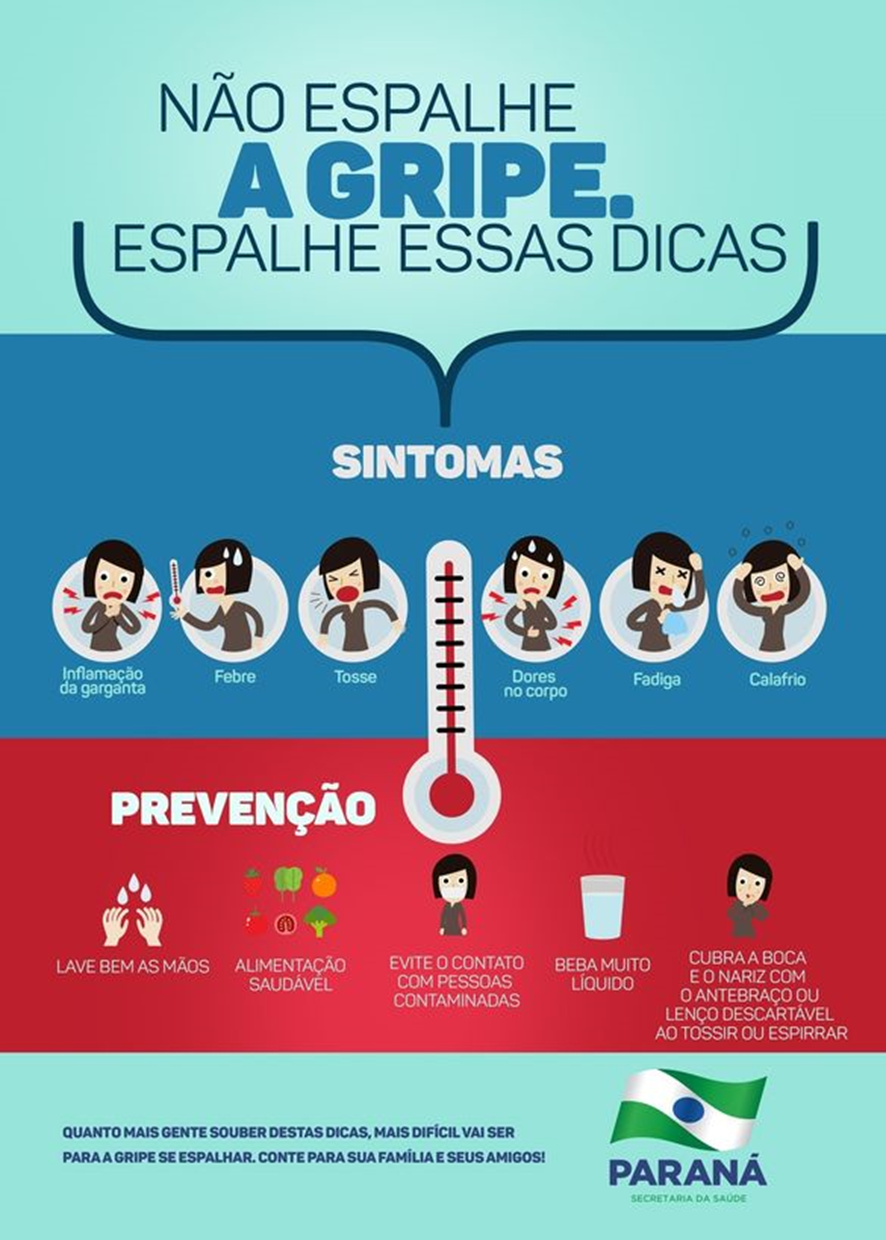
\includegraphics[width=.7\textwidth]{media/image19.png}
\end{figure}
%SECRETARIA DA SAÚDE DO PARANÁ. Governo lança campanha para estimular prevenção de gripe. Disponível em: \textless{}www.saude.pr.gov.br/modules/noticias/article.php?storyid=4950\textgreater{}. Acesso em: 7 mar. 2023.

A finalidade dessa campanha é

%Fábia e Felipe: alterei as alternativas porque duas delas me pareceram ``pegadinhas''
%Paulo, detalhe importante: o link apresentado pelo autor não existe mais. Encontrei o cartaz no link a seguir: http://www.crfpr.org.br/noticia/visualizar/id/7066#:~:text=Preocupado%20com%20o%20aumento%20do,sintomas%20que%20caracterizam%20a%20doen%C3%A7a. 

\begin{escolha}
\item apresentar ao público sugestões de alimentação saudável.

\item conscientizar a respeito da importância de beber água.

\item motivar o isolamento social das pessoas que estão gripadas.

\item informar sobre sintomas e sugerir dicas de prevenção contra gripe.
\end{escolha}


\chapter{Notícias}
\markboth{Módulo 5}{}

%\coment{Neste módulo, espera-se que os alunos leiam e compreendam textos do campo da vida pública; infiram significado de expressões apresentadas no título do capítulo; identifiquem elementos apresentados no primeiro parágrafo da notícia (antecipação sobre o fato); estabeleçam expectativas em relação ao texto a ser lido com base nos conhecimentos prévios; observem manchetes de jornais e reconheçam suas características e função no texto.}

\colorsec{Habilidades do SAEB}

\begin{itemize}
  \item Reconhecer diferentes modos de organização composicional de textos em versos.

  \item Analisar a construção de sentidos de textos em versos com base em seus elementos constitutivos.
\end{itemize}

%https://br.freepik.com/vetores-gratis/pessoas-sem-rosto-com-jornais\_23822995.htm\#page=2\&query=manchete\&position=31\&from\_view=keyword\&track=sph

\colorsec{Habilidade da BNCC}

\begin{itemize}
	\item 
 EF35LP16
\end{itemize}

\conteudo{
\textbf{NOTÍCIAS}

A \textbf{notícia} é um gênero textual muito presente no
cotidiano das pessoas. Sua finalidade é informar sobre fatos e
acontecimentos de relevância da atualidade que aconteceram nos mais
variados locais, que normalmente interessam a grande parte da população.

As notícias são veiculadas nos meios de comunicação por meio da
\textbf{escrita} --- em jornais e revistas impressos --- ou da \textbf{fala},
como ocorre em noticiários da televisão, do rádio e da internet.

Seja qual for o formato, as notícias costumam ser acompanhadas por
\textbf{imagens} (fotos, mapas, infográficos ou vídeos). De acordo com o
público-alvo ou o assunto a ser abordado, a notícia pode apresentar tanto a
linguagem formal como a informal.

Ao escrever uma notícia, é importante lembrar-se de que seu principal
objetivo é transmitir informações de modo claro e objetivo. Assim sendo,
é fundamental deixar claro no texto qual fato é noticiado e com quem, quando,
onde, como e por que esse fato aconteceu.

A notícia apresenta uma estrutura bem definida, que deve conter: título,
lide e corpo da notícia. O \textbf{título}, que abre a notícia, normalmente,
deve ser chamativo e apresentar os elementos fundamentais que serão relatados.
A \textbf{lide} é um pequeno texto que aborda ou resume os principais temas de 
uma matéria jornalística. O \textbf{corpo da notícia} é o texto informativo, 
que explora em detalhes o que foi apresentado de maneira geral no título e na
lide. 

\noindent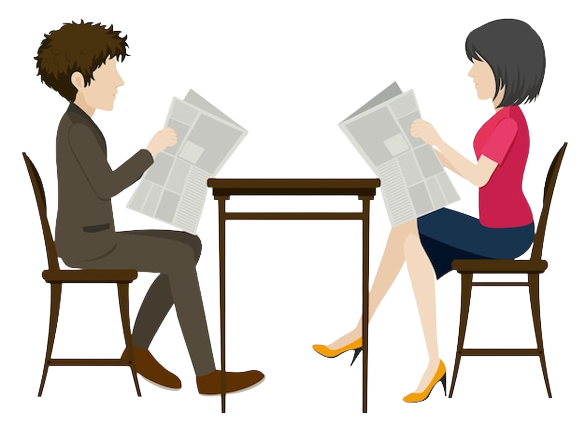
\includegraphics[width=\textwidth]{media/image20.png}}

\colorsec{Atividades}

\num{1} Leia esta notícia.

%07/06/2022

%\href{https://observatorio3setor.org.br/author/maria-fernanda-garcia/}{MARIA FERNANDA GARCIA}~ \href{https://observatorio3setor.org.br/category/noticias/mundo/}{MUNDO}~\href{https://observatorio3setor.org.br/category/noticias/}{NOTÍCIAS}

\begin{quote}
\textbf{Milagre: menino de 4 anos sobrevive sozinho por 2 dias em mata densa e fria}

\emph{Ryker Webb, de 4 anos, foi encontrado após passar dois dias
sozinho em uma área de mata com baixas temperaturas, em Montana, nos
EUA. Segundo as autoridades, cerca de 53 pessoas se empenharam nas
buscas do menino}

Ryker Webb, de 4 anos, foi encontrado após passar dois dias sozinho em
uma área de mata com baixas temperaturas, no estado de Montana, nos
Estados Unidos.

O menino desapareceu na última sexta-feira (03/06) e foi encontrado no
domingo (05/06) após um grande esforço que envolveu equipes de
socorristas, drones, helicópteros e barcos. Quando foi localizado, Webb
estava ileso, mas ``faminto, com sede e frio'', segundo o texto que o
Gabinete do Xerife do Condado de Lincoln publicou em sua página no
Facebook.

As autoridades enviaram um ``código vermelho'' de alerta a todos os
vizinhos da família Webb, pedindo a eles que procurassem a criança em
suas propriedades.

O pequeno Ryker estava brincando com o cachorro de sua família, no
quintal da casa onde mora, quando de repente desapareceu. Ele foi
encontrado a cerca de 3,8 km do local, depois de enfrentar a temperatura
de 4°C e chuvas fortes, que atrapalharam o trabalho das equipes de
resgate.

O Gabinete do Xerife local ainda ressaltou que a vegetação densa da área
tornou a busca ``extremamente difícil''. Quando a criança foi
localizada, 53 pessoas estavam empenhadas no trabalho
de resgate na
região. Autoridades e voluntários consideraram um verdadeiro milagre o
pequeno conseguir sobreviver em um terreno tão hostil com baixas
temperaturas.

\fonte{Maria Fernanda Garcia. Observatório do terceiro setor. Milagre: menino de 4 anos sobrevive sozinho por 2 dias em mata densa e fria. Disponível em:
https://observatorio3setor.org.br/noticias/milagre-menino-de-4-anos-sobrevive-sozinho-por-2-dias-em-mata-densa-e-fria/.
Acesso em: 07 mar. 2023.}
\end{quote}

\begin{escolha}
\item Que fato é relatado na notícia?

\reduline{Na notícia, relata-se que um menino de 4 anos sobreviveu sozinho por 2 dias em mata densa e fria, no Estado de Montana, nos Estados Unidos.\hfill}

\pagebreak
\item Onde o fato relatado aconteceu?

\reduline{O fato aconteceu em Montana, nos EUA.\hfill}
\linhas{1}

\item Quando o fato aconteceu?

\reduline{O menino desapareceu na sexta-feira, 03/06, e foi encontrado no 
domingo, 05/06.\hfill}
\linhas{3}

\item
  Sublinhe o trecho do texto que você usou para responder à questão anterior.

\coment{Resposta pessoal. Espera-se que os alunos sublinhem o segundo parágrafo do texto.}

\item Quem são os envolvidos no fato?

\reduline{Os envolvidos no fato são Ryker Webb, equipes de socorristas,
autoridades e voluntários.\hfill}
\linhas{2}

\item Onde a notícia foi publicada?

\reduline{A notícia foi publicada no site Observatório do terceiro setor.\hfill}
\linhas{1}

\item Quem escreveu a notícia?

\reduline{A autora da notícia é Maria Fernanda Garcia\hfill}
\linhas{1}

\item Essa notícia foi escrita para quem?

\reduline{Espera-se que os alunos percebam que a notícia é destinada a
quaisquer leitores interessados no conteúdo divulgado.\hfill}
\linhas{2}

\item Por você acha que esse fato virou notícia?

\reduline{Resposta pessoal.
Espera-se que os alunos percebam que o fato virou notícia porque não é
comum um menino de 4 anos sobreviver sozinho por 2 dias em mata densa e
fria.\hfill}
\linhas{1}
\end{escolha}

\num{2} Releia o título da notícia e o texto que vem após o título.

\begin{quote}
\textbf{Milagre: menino de 4 anos sobrevive sozinho por 2 dias em mata densa e fria}

\emph{Ryker Webb, de 4 anos, foi encontrado após passar dois dias
sozinho em uma área de mata com baixas temperaturas, em Montana, nos
EUA. Segundo as autoridades, cerca de 53 pessoas se empenharam nas
buscas do menino}
\end{quote}

\begin{escolha}
\item Os títulos dos textos jornalísticos são denominados de \reduline{manchete\hfill}.

\item Qual é a função da manchete? Marque a(s) alternativa(s) correta(s).

\begin{boxlist}
\boxitem{X} Chamar a atenção do leitor para o assunto da notícia.

\boxitem{\white{X}} Narrar a notícia.

\boxitem{X} Mostrar qual será o assunto tratado.
\end{boxlist}

\item Elabore um novo título para essa notícia.

\reduline{Sugere-se que os alunos compartilhem as respostas, averiguando
a coerência do título criado por eles com o tema da notícia.\hfill}
\end{escolha}

\colorsec{Treino}

\num{1} Leia o texto a seguir.
%(Fácil)

\begin{quote}
\textbf{Canudo sustentável de bambu ganha adeptos no AC e engenheiro
recebe até 500 encomendas de kits por mês}

O canudo plástico parece inofensivo, mas virou um vilão para o meio
ambiente, porque não é biodegradável e leva centenas de anos para se
decompor. {[}...{]}

Em 2019, o Acre aprovou uma lei --- ainda sem regulamentação ---
proibindo o canudo plástico.

No estado acreano, uma alternativa sustentável, leve, durável, prática e
reutilizável vem ganhando adeptos: o canudo de bambu. Em seis meses, o
agrônomo Emanuel Amaral, que confecciona o canudo, viu a procura pelos
kits aumentar em até 400\%.

{[}...{]}

\fonte{Aline Nascimento. G1. Canudo sustentável de bambu ganha adeptos no AC e
engenheiro recebe até 500 encomendas de kits por mês. Disponível
em:
https://g1.globo.com/ac/acre/natureza/amazonia/noticia/2019/12/31/canudo-sustentavel-de-bambu-ganha-adeptos-no-ac-e-engenheiro-recebe-ate-500-encomendas-de-kits-por-mes.ghtml.
Acesso em: 25 abr. 2023.}
\end{quote}

O texto pertence ao gênero textual

\begin{escolha}
\item fábula, porque narra as experiências vividas pelo autora do texto no Acre.

\item notícia, porque informa sobre a substituição do canudo plástico pelo de bambu.

\item poema, porque mostra, por meio de versos, uma ação sustentável ocorrida no Acre.

\item conto, porque contém uma narrativa curta sobre a produção de canudos de bambu.
\end{escolha}



\num{2} Leia a notícia a seguir.
%(Médio)

\begin{quote}
\textbf{Defesas curiosas}

Para escapar dos seus inimigos, certos animais e vegetais possuem
maneiras curiosas para se defender. O gambá e o percevejo exalam mau
cheiro para afugentar seus atacantes. O ouriço-do-mar tem espinhos
protetores em volta do corpo. O polvo solta uma tinta que escurece a
água, facilitando assim a sua fuga. O cacto também tem espinhos
protetores. As flores do açafrão são parecidas com as de outra planta
chamada cólquico que, por ser venenosa, é evitada como alimento por
certos animais. Por causa dessa semelhança, o açafrão fica protegido
também.

\fonte{Ana Rosa Abreu e outros autores. Defesas curiosas. Alfabetização: 
livro do aluno, Vol.3: textos informativos, textos instrucionais e 
biografias. Disponível em:
www.dominiopublico.gov.br/download/texto/me000590.pdf. Acesso em: 25 abr.
2023.}
\end{quote}
\pagebreak

A finalidade da notícia apresentada é apresentar

\begin{escolha}
\item animais que atacam seus inimigos de maneira curiosa.

\item plantas inteligentes que provocam seus predadores.

\item animais que são mais espertos do plantas para se defender.

\item animais e plantas que se defendem de maneira curiosa.
\end{escolha}



\num{3} O texto a seguir traz informações sobre uma competição esportiva. 
Leia-o atentamente.

\begin{quote}
\textbf{Seleção masculina de vôlei estreia hoje na Liga das Nações}

A seleção masculina de voleibol estreia nesta sexta-feira
(31), na Liga das Nações, jogando em Katowice, na Polônia, contra a 
seleção dos Estados Unidos.
Esta é a primeira etapa de cinco envolvendo 16 equipes. No grupo de 
Katowice estão Brasil, Estados Unidos, Austrália e Polônia. Todos as 16
seleções jogam entre si e em cada etapa mudam os adversários e a cidade 
sede.

\fonte{Eurico Tavares. Seleção masculina de vôlei estreia hoje na Liga das
Nações. RadioagênciaNacional. Disponível em:
http://radioagencianacional.ebc.com.br/geral/audio/2019-05/selecao-masculina-de-volei-estreia-hoje-na-liga-das-nacoes.
Acesso em: 25 abr. 2023.}
\end{quote}

Com base nas características apresentadas, pode-se afirmar que o texto
acima é 

\begin{escolha}
\item entrevista.

\item notícia.

\item diário.

\item conto.
\end{escolha}



\chapter{Discurso Direto}
\markboth{Módulo 6}{}

%\coment{Neste módulo, os alunos vão reconhecer os efeitos dos verbos de enunciação no discurso direto, percebendo a importância desses verbos para indicar os turnos de fala dos diálogos e para especificar entonações e sentidos das falas das personagens.}

\conteudo{
\textbf{Verbos de enunciação e variedades linguísticas no discurso direto}

%https://pixabay.com/pt/illustrations/gabarito-relat\%c3\%b3rio-de-volta-3387220/
\noindent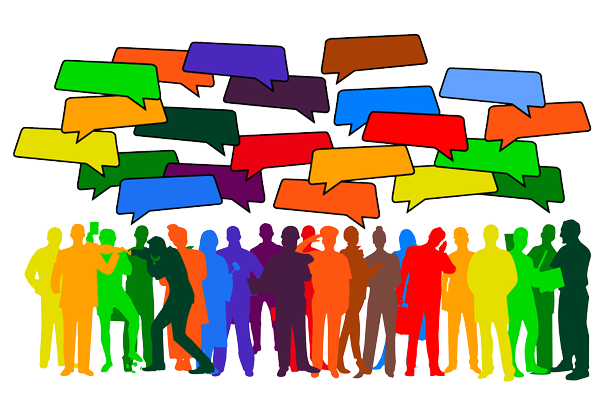
\includegraphics[width=\textwidth]{media/image21.png}

Na língua portuguesa, há palavras que anunciam quando um personagem vai falar e o modo como vai falar, por exemplo: ``disse'', ``perguntou'', ``respondeu''.

Observe este exemplo:

\begin{quote}
--- Eu não falei? Ele sempre volta! --- \textbf{disse} o dono do cachorro.
\end{quote}

Essas palavras podem ser encontradas antes, no meio ou depois das falas
da personagem e são chamados de \textbf{verbos de enunciação/elocução}. 
Estes são verbos utilizados no texto que servem para introduzir/iniciar 
a fala dos personagens, indicando suas atitudes e ações. Além disso, podemos
observar que as falas das personagens podem ser introduzidas
seguidas de dois-pontos e travessão, em forma de diálogo. Esses
elementos são importantes, pois ajudam a compreender formas e intenções
das personagens nos diálogos.

Agora, vamos treinar!
}

\colorsec{Atividades}

\num{1} Leia o texto a seguir.

%https://pixabay.com/pt/illustrations/lobo-fera-lobo-cinza-animal-6612744/

\begin{quote}
\begin{wrapfigure}{r}{.5\textwidth}
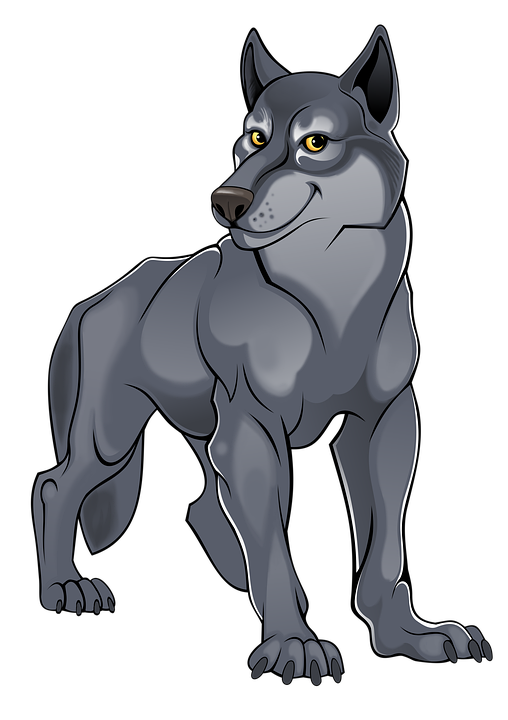
\includegraphics[width=.5\textwidth]{media/image22.png}
\end{wrapfigure}

\textbf{O lobo e o cão}

Um lobo e um cão se encontraram num caminho. Disse o lobo:

--- Companheiro, você está com ótimo aspecto: gordo, o pelo
lustroso\ldots{} Estou até com inveja!

--- Ora, faça como eu --- respondeu o cão. --- Arranje um bom amo. Eu
tenho comida na hora certa, sou bem tratado\ldots{} Minha única
obrigação é latir à noite, quando aparecem ladrões. Venha comigo e você
terá o mesmo tratamento.

O lobo achou ótima a ideia e se puseram a caminho.

Mas, de repente, o lobo reparou numa coisa. --- O que é isso no seu
pescoço, amigo? Parece um pouco esfolado\ldots{} --- observou ele.

--- Bem --- disse o cão --- isso é da coleira. Sabe? Durante o dia,
meu amo me prende com uma coleira, que é para eu não assustar as pessoas
que vêm visitá-lo.

O lobo se despediu do amigo ali mesmo:

--- Vamos esquecer --- disse ele. --- Prefiro minha liberdade à sua
fartura.

\fonte{Ana Rosa Abreu e outros autores. O lobo e o cão. Alfabetização, Vol.2:
contos, fábulas, lendas e mitos. Disponível em:
www.dominiopublico.gov.br/download/texto/me000589.pdf.
Acesso em: 24 abr. 2023.}
\end{quote}

\begin{tabular}{ll}
\textbf{Glossário} & \mbox{}\\
Amo & dono do cão\\
Cativo & preso\\
Esfolado & machucado\\
Lustroso & brilhante\\
\end{tabular}

\begin{escolha}
\item Quem são as personagens da história?

\reduline{As personagens são o cão e o lobo.\hfill}

\item O texto que você acabou de ler é do gênero:

\begin{boxlist}
\boxitem{\white{X}} diário, texto pessoal em que uma pessoa relata experiências e reflexões.

\boxitem{X} fábula, narrativa concluída com moral da história, em que animais agem como gente.

\boxitem{\white{X}} notícia, texto de jornal que apresenta um acontecimento real para o grande público.
\end{boxlist}

\item Qual convite o lobo recebeu do cão?

\reduline{O cão convidou o lobo a viver com ele.\hfill}
\linhas{1}

\item Por que o lobo desistiu do convite?

\reduline{O lobo desistiu do convite depois de ver as marcas da coleira no pescoço do cão.\hfill}
\linhas{2}

\item Descreva o conflito principal da fábula.

\reduline{No texto, o cão é bem tratado pelo seu tutor, mas não tem a liberdade
do lobo, isto é: o desfrute da plena liberdade se opõe às regalias de abrir 
mão dela.\hfill}
\end{escolha}

\num{2} Quem conta a história \textbf{O lobo e o cão}? Assinale a alternativa correta.

\begin{boxlist}
\boxitem{\white{X}} Um narrador que participa da história (narração em 1ª pessoa).

\boxitem{X} Um narrador que não participa das ações (narração em 3ª pessoa).
\end{boxlist}

\num{3} No trecho a seguir, quem está participando do diálogo?

\begin{quote}
--- Companheiro, você está com ótimo aspecto: gordo, o pelo
lustroso\ldots{} Estou até com inveja!

--- Ora, faça como eu --- respondeu o cão. --- Arranje um bom amo. Eu
tenho comida na hora certa, sou bem tratado\ldots{} Minha única
obrigação é latir à noite, quando aparecem ladrões. Venha comigo e você
terá o mesmo tratamento.
\end{quote}

\reduline{A primeira das duas falas é do lobo; a segunda é do cão.\hfill}
\linhas{1}

\pagebreak
\num{4} Como ficaria a história se o diálogo fosse composto apenas pelas falas
das personagens, sem a intervenção do narrador?

\reduline{Resposta pessoal. Espera-se que os alunos percebam que o leitor não
saberia de que maneira as personagens falaram, pois não haveria os
comentários, nem os verbos de enunciação.\hfill}

\reduline{Explique aos alunos que, em algumas narrativas, pode acontecer de o
narrador não indicar quem fala; a identificação é feita pela sequência
do discurso e a apresentação pelos verbos de enunciação.\hfill}

\num{5} Releia a fábula e pinte no texto:

\begin{itemize}
\item de azul as falas do cão;

\item de verde as falas do lobo.
\end{itemize}

\num{6} Qual o efeito obtido por meio do discurso direto na fábula ``\textbf{O lobo e o cão''}?

\reduline{Espera-se que os alunos percebam que o discurso direto apresenta
ao leitor a conversa das personagens como se estivesse ocorrendo naquele
momento.\hfill}

\colorsec{Treino}

\num{1} Leia o trecho do conto ``Água da vida'', observando atentamente 
os diálogos.

%(Fácil)

\begin{quote}
\textbf{Água da vida}

Houve, uma vez, um rei muito poderoso, que vivia feliz e tranquilo em
seu reino. Um belo dia, adoeceu gravemente e ninguém tinha esperanças de
que escapasse. Ele tinha três filhos, {[}...{]}.

Encontravam-se eles no jardim do castelo a chorar e, de repente, viram
surgir à sua frente um velho de aspecto venerável, que indagou a causa
de tamanha tristeza. Disseram-lhe que estavam aflitos porque o pai
estava gravemente enfermo e os médicos já não tinham esperanças de o
salvar.

O velho, então, disse-lhe:

--- Eu conheço um remédio muito eficaz, que poderá curá-lo; é a famosa
Água da Vida. Mas é muito difícil obtê-la.

\fonte{Irmãos Grimm. A água da vida. Contos de Grimm. Disponível em:
https://www.grimmstories.com/pt/grimm\_contos/a\_agua\_da\_vida. Acesso
em: 25 abr. 2023.}
\end{quote}

O trecho ``--- Eu conheço um remédio muito eficaz, que poderá curá-lo; é a
famosa Água da Vida. Mas é muito difícil obtê-la'' está em discurso

\begin{escolha}
\item direto, porque é a fala do personagem separada por travessão.

\item indireto, porque é a fala do personagem por meio do narrador.

\item direto, porque é a transcrição da fala do próprio narrador do conto.

\item indireto, porque apresenta a introdução do narrador ``disse-lhe''.
\end{escolha}

\num{2} No diálogo a seguir, do livro \textit{O mágico de Oz}, a personagem
Dorothy e a Bruxa do Norte estão conversando.

%(Médio) 

\begin{quote}
--- Eu sempre acreditei que todas as bruxas fossem más --- disse a menina,
que sentia medo por estar frente a frente com uma bruxa de verdade.

--- Oh, não, não, isso é um erro! Havia quatro bruxas na Terra de Oz: as
que vivem no Norte e no Sul são boas, as do Leste e do Oeste eram bruxas
malvadas, mas agora que você matou uma delas sobrou apenas uma bruxa má
em toda a Terra de Oz: a que vive no Reino do Oeste.

Depois de pensar um pouco, Dorothy disse:

--- Mas a tia Ema me contou que todas as bruxas morreram há muitos e
muitos anos.

--- Quem é a tia Ema? --- perguntou a bruxinha.

--- É a minha tia que mora no Kansas, eu vim de lá.

%Suponho que o autor do material tenha feito a tradução, porque o livro citado abaixo está em inglês.
\fonte{Frank L. Baum. O mundo mágico de OZ. Tradução feita para este material. Disponível em:
www.dominiopublico.gov.br/download/texto/ph000102.pdf. Acesso em: 25 abr.
2023.}
\end{quote}

No trecho ``--- Oh, não, não, isso é um erro!'', o uso de ``oh'' indica

\begin{escolha}
\item alegria.

\item surpresa.

\item alívio.

\item tristeza.
\end{escolha}

\num{3} O livro \textit{Viagem ao centro da Terra}, escrito por Júlio Verne e
publicado em 1864, é o relato do jovem Axel sobre a jornada que
percorreu com o seu tio. O diálogo a seguir refere-se a uma discussão
acerca da continuidade da expedição.
%(Difícil) 

\begin{quote}
{[}...{]}

--- Oh, não tenho medo de que o céu nos caia sobre a cabeça. Agora, meu
tio, quais são seus planos? O senhor não está pensando em voltar à
superfície do globo?

--- Voltar? Ora essa! Muito pelo contrário, pretendo continuar a viagem
já que tudo correu tão bem até aqui.

--- É que não vejo como atravessaremos essa planície líquida.

--- Não pretendo mergulhar de cabeça.
\end{quote}

\fonte{Júlio Verne. Viagem ao centro da Terra. Disponível em:
www.ebc.com.br/sites/\_portalebc2014/files/atoms/files/viagem\_ao\_centro\_da\_terra\_\_julio\_verne.pdf.
Acesso em: 25 abr. 2023.}

No trecho de diálogo entre tio e sobrinho, prevalece

\begin{escolha}
\item a linguagem jovem, com gírias.

\item a linguagem das crianças, com diminutivos.

\item a linguagem científica, com termos específicos.

\item a norma-padrão, com certa formalidade.
\end{escolha}

\chapter{Concordância nominal}
\markboth{Módulo 7}{}

%\coment{Neste módulo, os alunos vão identificar, no texto, os adjetivos e os substantivos a que se referem; perceber a concordância em número e gênero entre artigo, substantivo e adjetivo; aplicar a concordância nominal nos diversos contextos para corresponder à norma-padrão.}

\conteudo{
\textbf{Concordância nominal}\bigskip

%https://pixabay.com/pt/illustrations/abc-alfabeto-letras-ler-aprender-916665/
\noindent
\includegraphics[width=\textwidth]{media/image23.png}

Imagine a confusão que seria a comunicação se as pessoas ou os objetos
não tivessem nomes para identificá-los.

\textbf{Substantivo} é o nome de cada coisa que existe no planeta. Há
variadas formas de atribuir qualidade a um substantivo. Por exemplo: 
uma camiseta pode ser branca, preta, azul, amarela (ou de muitas outras
cores); quanto ao tamanho, a mesma peça de roupa pode ser curta ou comprida.
E também podemos dizer que ela é barata ou cara, em relação ao preço.

As palavras que servem para atribuir noções de qualidade, 
natureza, estado, e outras, ao substantivo são 
chamadas de\textbf{adjetivos}.

Importante saber que o \textbf{substantivo} pode variar em
\textbf{gênero} (masculino ou feminino) e \textbf{número} (singular ou
plural). O \textbf{adjetivo} e o \textbf{artigo} devem concordar em
gênero e número com o substantivo a que se referem.
}

\colorsec{Atividades}

Conto é um gênero narrativo muito popular na literatura. Geralmente, 
os contos são narrativas curtas, em que as ações contadas por um 
narrador e são vividas por uma ou mais personagens, em um lugar e 
período específicos.  

%\coment{Chame a atenção dos alunos para o título do texto: ``O soldadinho de chumbo''. Peça a eles que levantem hipóteses sobre o enredo com base no título. Provavelmente, alguns farão referência a um enredo de conto de fadas. Incentive a participação dos alunos.}

\num{1} Leia o conto Joãozinho-sem-medo e, em seguida, responda às questões propostas.

%https://br.freepik.com/vetores-gratis/guarda-em-pe-com-uma-arma\_13571969.htm\#query=soldadinho\%20chumbo\&position=3\&from\_view=search\&track=ais

\begin{quote}
\textbf{O Soldadinho de Chumbo}

%Fábia e Felipe: esse conto é muito mais extenso do que qualquer outro texto deste volume e de todos os outros que editei. Parece-me que esse tamanho escapa ao padrão do nosso material. 



Numa loja de brinquedos havia uma caixa de papelão com vinte e cinco
soldadinhos de chumbo, todos iguaizinhos, pois haviam sido feitos com o
mesmo molde. Apenas um deles não estava inteiro: como fora o último a ser
fundido, faltou chumbo para completar-lhe uma das pernas. Mas esse soldadinho
logo aprendeu a ficar em pé sobre a perna que tinha e não fazia feio
ao lado dos irmãos.

Esses soldadinhos de chumbo eram muito bonitos e elegantes, cada qual
com seu fuzil ao ombro, a túnica escarlate, calça azul e uma bela pluma
no chapéu. Além disso, tinham feições de soldados corajosos e
cumpridores do dever.

Os valorosos soldadinhos de chumbo aguardavam o momento em que passariam
a pertencer a algum menino.

Chegou o dia em que a caixa foi dada de presente de aniversário a um
garoto. Foi o presente de que ele mais gostou:

--- Que lindos soldadinhos! --- exclamou maravilhado.

E os colocou enfileirados sobre a mesa, ao lado dos outros brinquedos. O
soldadinho de uma perna só era o último da fileira.

Ao lado do pelotão de chumbo se erguia um lindo castelo de papelão, um
bosque de árvores verdinhas e, em frente, havia um pequeno lago feito de
um pedaço de espelho.

\begin{wrapfigure}{r}{.5\textwidth}

\includegraphics[width=.5\textwidth]{media/image24.png}
\end{wrapfigure}

A maior beleza, porém, era uma jovem que estava em pé na porta do
castelo. Ela também era de papel, mas vestia uma saia de tule bem
franzida e uma blusa bem justa. Seu lindo rostinho era emoldurado por
longos cabelos negros, presos por uma tiara enfeitada com uma pequenina
pedra azul.

A atraente jovem era uma bailarina, por isso mantinha os braços erguidos
em arco sobre a cabeça. Com uma das pernas dobrada para trás, tão
dobrada, mas tão dobrada, que acabava escondida pela saia de tule.

O soldadinho a olhou longamente e logo se apaixonou, e pensando que, tal
como ele, aquela jovem tão linda tivesse uma perna só.

``Mas é claro que ela não vai me querer para marido'', pensou
entristecido o soldadinho, suspirando. ``Tão elegante, tão
bonita\ldots{} Deve ser uma princesa. E eu? Nem cabo sou, vivo numa
caixa de papelão, junto com meus vinte e quatro
irmãos''.

À noite, antes de deitar, o menino guardou os soldadinhos na caixa, mas
não percebeu que aquele de uma perna só caíra atrás de uma grande
cigarreira.

Quando os ponteiros do relógio marcaram meia-noite, todos os brinquedos
se animaram e começaram a aprontar mil e uma. Uma enorme bagunça!

As bonecas organizaram um baile, enquanto o giz da lousa desenhava
bonequinhos nas paredes. Os soldadinhos de chumbo, fechados na caixa,
golpeavam a tampa para sair e participar da festa, mas continuavam
prisioneiros.

Mas o soldadinho de uma perna só e a bailarina não saíram do lugar em
que haviam sido colocados. Ele não conseguia parar de olhar aquela
maravilhosa criatura. Queria ao menos tentar conhecê-la, para ficarem
amigos.

De repente, se ergueu da cigarreira um homenzinho muito mal-encarado.
Era um gênio ruim, que só vivia pensando em maldades. Assim que ele
apareceu, todos os brinquedos pararam amedrontados, pois já sabiam de
quem se tratava.

O geniozinho olhou a sua volta e viu o soldadinho, deitado atrás da
cigarreira.

--- Ei, você aí, por que não está na caixa, com seus irmãos? --- gritou
o monstrinho.

Fingindo não escutar, o soldadinho continuou imóvel, sem desviar os
olhos da bailarina.

--- Amanhã vou dar um jeito em você, você vai ver! --- Gritou o geniozinho
enfezado. --- Pode esperar.

Depois disso, pulou de cabeça na cigarreira, levantando uma nuvem que
fez todos espirrarem.

Na manhã seguinte, o menino tirou os soldadinhos de chumbo da caixa,
recolheu aquele de uma perna só, que estava caído atrás da cigarreira, e
os arrumou perto da janela. O soldadinho de uma perna só, como de
costume, era o último da fila.

De repente, a janela se abriu, batendo fortemente as venezianas. Teria
sido o vento, ou o geniozinho maldoso? E o pobre soldadinho caiu de
cabeça na rua.

O menino viu quando o brinquedo caiu pela janela e foi correndo
procurá-lo na rua. Mas não o encontrou. Logo se consolou: afinal, tinha
ainda os outros soldadinhos, e todos com duas pernas.

Para piorar a situação, caiu um verdadeiro temporal. Quando a tempestade
foi cessando, e o céu limpou um pouco, chegaram dois moleques. Eles se
divertiam, pisando com os pés descalços nas poças de água. Um deles viu
o soldadinho de chumbo e exclamou:

--- Olhe! Um soldadinho! Será que alguém jogou fora porque ele está
quebrado?

--- É, está um pouco amassado. Deve ter vindo com a enxurrada.

--- Não, ele está só um pouco sujo.

--- O que nós vamos fazer com um soldadinho só? Precisaríamos pelo menos
meia dúzia, para organizar uma batalha.

--- Sabe de uma coisa? --- Disse o primeiro garoto. --- Vamos colocá-lo
num barco e mandá-lo dar a volta ao mundo.

E assim foi. Construíram um barquinho com uma folha de jornal, colocaram
o soldadinho dentro dele e soltaram o barco para navegar na água que
corria pela sarjeta.

Apoiado em sua única perna, com o fuzil ao ombro, o soldadinho de chumbo
procurava manter o equilíbrio. O barquinho dava saltos e esbarrões na
água lamacenta, acompanhado pelos olhares dos dois moleques que,
entusiasmados com a nova brincadeira, corriam pela calçada ao lado.

Lá pelas tantas, o barquinho foi jogado para dentro de um bueiro e
continuou seu caminho, agora subterrâneo, em uma imensa escuridão. Com o
coração batendo fortemente, o soldadinho voltava todos seus pensamentos
para a bailarina, que talvez nunca mais pudesse ver.

De repente, viu chegar em sua direção um enorme rato de esgoto, olhos
fosforescente e um horrível rabo fino e comprido, que foi logo
perguntando:

--- Você tem autorização para navegar? Então? Ande, mostre-a logo, sem
discutir.

O soldadinho não respondeu, e o barquinho continuou seu incerto caminho,
arrastado pela correnteza. Os gritos do rato do esgoto exigindo a
autorização foram ficando cada vez mais distantes.

Enfim, o soldadinho viu ao longe uma luz, e respirou aliviado; aquela
viagem no escuro não o agradava nem um pouco. Mal sabia ele que,
infelizmente, seus problemas não haviam acabado.

A água do esgoto chegara a um rio, com um grande salto; rapidamente, as
águas agitadas viraram o frágil barquinho de papel.

O barquinho virou, e o soldadinho de chumbo afundou. Mal tinha chegado
ao fundo, apareceu um enorme peixe que, abrindo a boca, engoliu-o.

O soldadinho se viu novamente numa imensa escuridão, espremido no
estômago do peixe. E não deixava de pensar em sua amada: ``O que estará
fazendo agora sua linda bailarina? Será que ainda se lembra de mim?''.

E, se não fosse tão destemido, teria chorado lágrimas de chumbo, pois
seu coração sofria de paixão.

Passou-se muito tempo --- quem poderia dizer quanto?

E, de repente, a escuridão desapareceu e ele ouviu quando falavam:

--- Olhe! O soldadinho de chumbo que caiu da janela!

Sabem o que aconteceu? O peixe havia sido fisgado por um pescador,
levado ao mercado e vendido a uma cozinheira. E, por cúmulo da
coincidência, não era qualquer cozinheira, mas sim a que trabalhava na
casa do menino que ganhara o soldadinho no aniversário. Ao limpar o
peixe, a cozinheira encontrara dentro dele o soldadinho, do qual se
lembrava muito bem, por causa daquela única perna.

Levou-o para o garotinho, que fez a maior festa ao revê-lo. Lavou-o com
água e sabão, para tirar o fedor de peixe, e endireitou a ponta do
fuzil, que amassara um pouco durante aquela aventura.

Limpinho e lustroso, o soldadinho foi colocado sobre a mesma mesa em que
estava antes de voar pela janela. Nada estava mudado. O castelo de
papel, o pequeno bosque de árvores muito verdes, o lago reluzente feito
de espelho. E, na porta do castelo, lá estava ela, a bailarina: sobre
uma perna só, com os braços erguidos acima da cabeça, mais bela do que
nunca.

O soldadinho olhou para a bailarina, ainda mais apaixonado, ela olhou
para ele, mas não trocaram palavra alguma. Ele desejava conversar, mas
não ousava. Sentia-se feliz apenas por estar novamente perto dela e
poder amá-la.

Se pudesse, ele contaria toda sua aventura; com certeza a linda
bailarina iria apreciar sua coragem. Quem sabe, até se casaria com
ele\ldots{}

Enquanto o soldadinho pensava em tudo isso, o garotinho brincava
tranquilo com o pião. De repente como foi, como não foi --- é caso de se
pensar se o geniozinho ruim da cigarreira não metera seu nariz ---, o
garotinho agarrou o soldadinho de chumbo e atirou-o na lareira, onde o
fogo ardia intensamente.

O pobre soldadinho viu a luz intensa e sentiu um forte calor. A única
perna estava amolecendo e a ponta do fuzil envergava para o lado. As
belas cores do uniforme, o vermelho escarlate da túnica e o azul da
calça perdiam suas tonalidades.

O soldadinho lançou um último olhar para a bailarina, que retribuiu com
silêncio e tristeza. Ele sentiu então que seu coração de chumbo começava
a derreter --- não só pelo calor, mas principalmente pelo amor que ardia
nele.

Naquele momento, a porta escancarou-se com violência, e uma rajada de
vento fez voar a bailarina de papel diretamente para a lareira, bem
junto ao soldadinho. Bastou uma labareda e ela desapareceu. O soldadinho
também se dissolveu completamente.

No dia seguinte, a arrumadeira, ao limpar a lareira, encontrou no meio
das cinzas um pequenino coração de chumbo: era tudo que restara do
soldadinho, fiel até o último instante ao seu grande amor.

Da pequena bailarina de papel só restou a minúscula pedra azul da tiara,
que antes brilhava em seus longos cabelos negros.

\fonte{Hans Christian Andersen. O soldadinho de chumbo. Alfabetização, Vol.2: contos, fábula, lendas e mitos. Disponível em:
www.dominiopublico.gov.br/download/texto/me000589.pdf.
Acesso em: 24 abr. 2023. com alterações}
\end{quote}

%Fábia e Felipe: aqui tomei a liberdade de fazer pequenas adaptações no primeiro parágrafo para evitar a palavra ``perneta'', que poderia ser considerada capacitismo. Me digam o que acham. Uma alternativa é deixar o termo como está e explicar em uma nota que ele não adequado.  

\begin{escolha}
\item Qual é o assunto do conto?

\reduline{O tema do conto são as aventuras de um soldadinho de chumbo
apaixonado por uma bailarina de papel.\hfill}

\item Onde se inicia a história?

\reduline{A história se inicia em uma loja de brinquedos.\hfill}
\linhas{1}

\item Como o Soldadinho foi parar na rua?

\reduline{O menino que era dono do Soldadinho decidiu arrumar a tropa na
janela. Mas, talvez por maldade do geniozinho da cigarreira, talvez por causa
de um vento forte, o Soldadinho acabou caindo na rua.\hfill}
\linhas{5}

\item Quem foi o primeiro a encontrar o Soldadinho de Chumbo?

\reduline{O primeiro a encontrar o Soldadinho de Chumbo foi um dos meninos que 
estava passando pela rua.\hfill}

\item O que os meninos fizeram com o Soldadinho de Chumbo?

\reduline{Os meninos fizeram um barco de papel e colocaram o soldado dentro, 
para ele dar a volta ao mundo.\hfill}
\linhas{3}

\item Quem engoliu o Soldadinho de Chumbo?

\reduline{O Soldadinho de Chumbo foi engolido por um peixe muito grande.\hfill}
\linhas{1}

\item Como o Soldadinho voltou para sua casa?

\reduline{O peixe que engoliu o Soldadinho de Chumbo foi comprado pela
cozinheira da família do menino. Ela encontrou o Soldadinho na barriga 
do peixe e o entregou ao seu primeiro dono.\hfill}
\linhas{2}

\item Qual é o fim da história?

\reduline{O Soldadinho de Chumbo é arremessado pelo menino na lareira, onde
derrete junto com a bailarina, que foi parar no fogo depois de um pé de vento.
\hfill}
\linhas{3}
\end{escolha}

\num{2} Releia um trecho do conto \textbf{O soldadinho de chumbo}.

\begin{quote}
Esses soldadinhos de chumbo eram muito bonitos e elegantes
\end{quote}

\begin{escolha}
\item
  Circule os adjetivos que aparecem neste trecho.

  \reduline{Os alunos devem circular os adjetivos \textit{bonitos} e 
  \textit{elegantes}.\hfill}

\item
  A quem esses adjetivos se referem?

  \reduline{Os adjetivos se referem aos soldadinhos de chumbo.\hfill}
  \linhas{1}

\item O verbo está no singular ou no plural? Justifique sua resposta.

\reduline{O verbo está no plural para concordar com o substantivo 
\textit{soldadinhos}.\hfill}
\linhas{2}
\end{escolha}

\num{3} Na frase ``Além disso, tinham feições de soldados corajosos'', qual é o
adjetivo usado para qualificar o substantivo?

\reduline{\textit{Corajosos} é o adjetivo usado para qualificar o substantivo.
\hfill}
\linhas{2}

\num{4} Por que o adjetivo está no plural e no masculino?

\reduline{O adjetivo está no plural e no masculino para concordar com o
substantivo \textit{soldados}, a que se refere.\hfill}
\linhas{1}

\pagebreak
\num{5} Leia esta frase.

\begin{mdframed}[linewidth=10pt,linecolor=salmao!20,backgroundcolor=salmao!20,roundcorner=20pt]
O pobre soldadinho viu a luz intensa e sentiu um forte calor.
\end{mdframed}

\begin{escolha}
\item Qual é a classe gramatical da palavra destacada?

\reduline{A palavra destacada é um artigo.\hfill}

\item A concordância obedece às mesmas regras que você identificou na
  atividade anterior? Justifique sua resposta.

\reduline{Sim, a concordância obedece às mesmas regras da
  atividade anterior, porque, da mesma maneira que o adjetivo, o artigo deve concordar com o substantivo tanto em gênero quanto em número.\hfill}
\end{escolha}

\colorsec{Treino}

\num{1} Leia um trecho de um conto popular.
%(Fácil) 

\begin{quote}
\textbf{Acoitrapa E Chuquilhanto}

Na cordilheira que fica em cima do vale de Yyucay, em Cusco,
pode-se ouvir todos os sons. O vento sopra com sua bocarra;
a manhã, obrigada a se levantar sempre antes dos outros,
boceja morta de sono; os pássaros, seus eternos namorados,
acordam cantando ao ouvi-la se espreguiçar.

De repente, silêncio. Acaba de chegar Acoitrapa, o
pastor de lhamas. Ele é \textbf{jovem} e \textbf{belo}. Toca a quena tão
docemente, que até as flores mais \textbf{tímidas} se abrem e
despontam entre os galhos das árvores para escutá-lo. 

\fonte{Ana Rosa Abreu e outros autores. Acoitrapa E Chuquilhanto.
Alfabetização, Vol.2: contos, fábulas, lendas e mitos. Disponível em:
www.dominiopublico.gov.br/download/texto/me000589.pdf.
Acesso em: 24 abr. 2023.}
\end{quote}

As palavras destacadas no texto são:

\begin{escolha}
\item substantivos.

\item adjetivos.

\item artigos.

\item numeral.
\end{escolha}

\num{2} Leia um trecho da lenda indígena ``As lágrimas de Potira''.
%(Médio) 

\begin{quote}
\textbf{As lágrimas de Potira}

Muito antes de os brancos atingirem os sertões de Goiás, em busca de
pedras preciosas, existiam por aquelas partes do Brasil muitos povos
indígenas, vivendo em paz ou em guerra e segundo suas crenças e hábitos.
Numa das aldeias, que por muito tempo manteve a harmonia com seus
vizinhos, viviam Potira, menina bela contemplada por Tupã com a formosura das
flores, e Itagibá, jovem forte e valente. 

\fonte{Ana Rosa Abreu e outros autores. As lágrimas de Potira.
Alfabetização, Vol.2: contos, fábulas, lendas e mitos. Disponível em:
www.dominiopublico.gov.br/download/texto/me000589.pdf.
Acesso em: 24 abr. 2023.}
\end{quote}

Uma das palavra utilizadas no texto para caracterizar Potira é o adjetivo

\begin{multicols}{2}
\begin{escolha}
\item ``formosura''.

\item ``valente''.

\item ``forte''.

\item ``bela''.
\end{escolha}
\end{multicols}

\pagebreak
\num{3} Leia um trecho do texto ``Bruxas incompreendidas'',
da revista \textit{Ciência Hoje das Crianças}.
%(Difícil) 

\begin{quote}
\textbf{Bruxas incompreendidas}

Aposto que você já ouviu falar que, se pegar em uma mariposa e colocar a
mão no olho, você fica cego. Vou dizer uma coisa com franqueza: isso é
um mito. Acusadas de serem feias, sem graça e \textbf{venenosas}, as
mariposas são bichos muito incompreendidos. Quanta injustiça!

\fonte{Bruxas incompreendidas. Ciência Hoje das Crianças. Disponível em:
https://chc.org.br/bruxas-incompreendidas/. Acesso em: 25 abr. 2023.}
\end{quote}

A palavra ``venenosas'', destacada no texto, está concordando com

\begin{escolha}
\item bichos.

\item feias.

\item mariposas.

\item injustiça.
\end{escolha}

\chapter{Fatos e Opiniões}
\markboth{Módulo 8}{}

%\coment{Neste módulo, espera-se que os alunos localizem informações explícitas no texto; façam distinção entre fato e opiniões em texto jornalístico; e identifiquem a função social do texto.}

%https://br.freepik.com/vetores-gratis/ilustracao-do-conceito-de-opiniao\_20547312.htm\#query=opini\%C3\%A3o\&position=9\&from\_view=search\&track=sph

\conteudo{
\textbf{Fato ou opinião?}

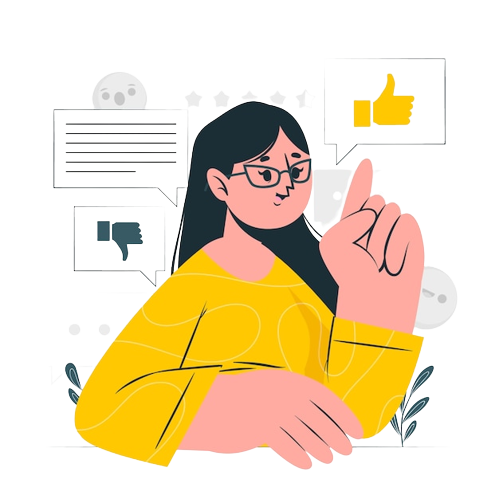
\includegraphics[width=\textwidth]{media/image25.png}

\textbf{Fato} é algo que ocorreu e pode ser comprovado de algum modo,
por meio de documentos, estatísticas, vídeos, estudos ou registros.
Observe o exemplo:

%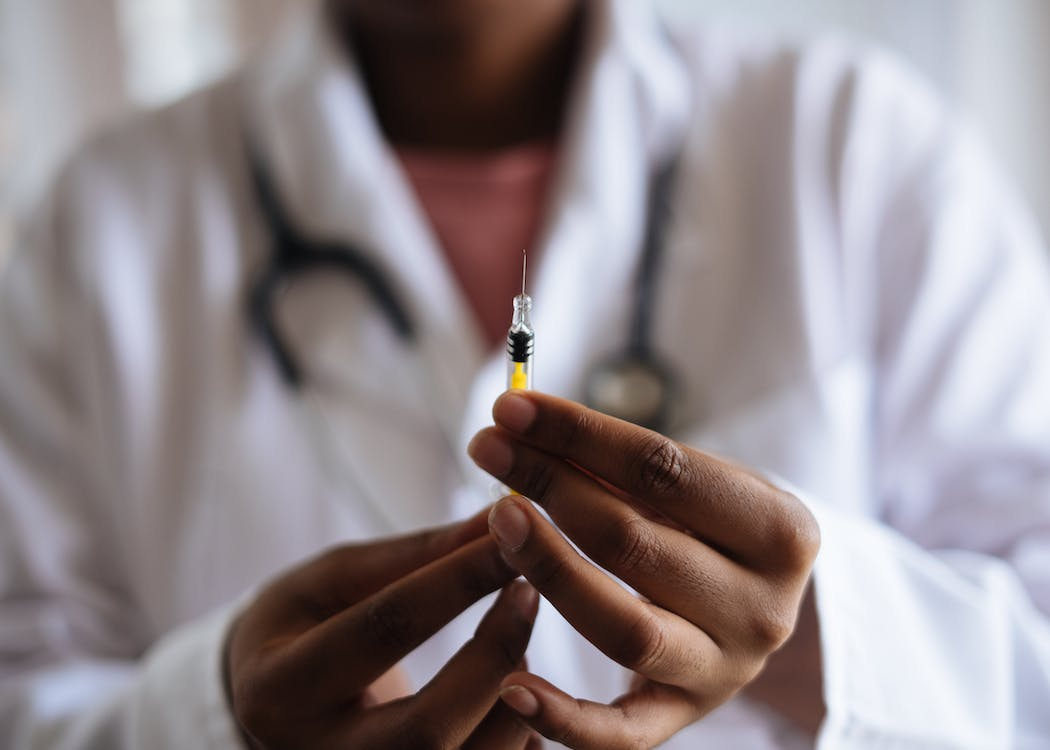
\includegraphics[width=\textwidth]{media/image26.jpeg}
%https://www.pexels.com/pt-br/foto/pessoa-segurando-injecao-3825529/
%Vacinas salvam vidas.

A informação é um fato, tendo em vista que há registros dos casos e, por
meio deles, é possível fazer uma afirmação.

\textbf{Opinião} consiste em uma interpretação do fato, isto é, uma
forma pessoal de olhar o fato. Essa opinião pode ser diferente de pessoa
para pessoa a depender de muitos fatores. Veja o exemplo:

%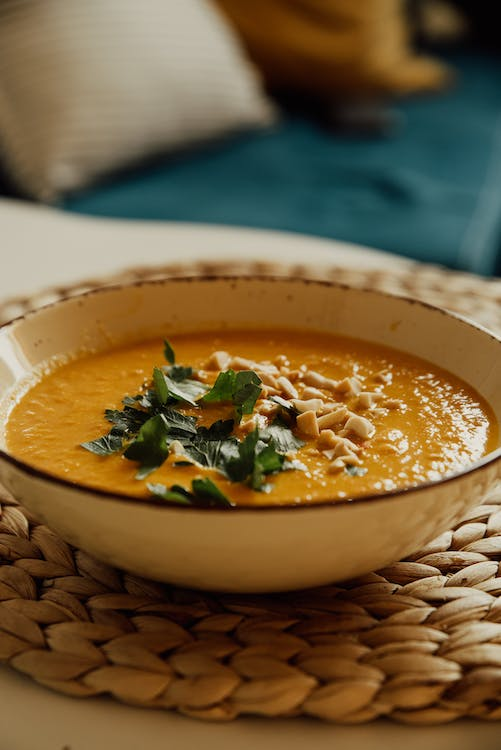
\includegraphics[width=\textwidth]{media/image27.jpeg}
%https://www.pexels.com/pt-br/foto/prato-de-sopa-em-tigela-de-ceramica-branca-6072108/
%Sopa é a melhor comida do mundo!
}

\colorsec{Atividades}

\num{1} Leia o texto a seguir.

%\coment{Realize a primeira leitura, em voz alta, até o fim do texto. Depois da sua leitura, solicite aos alunos que leiam alternadamente o texto. Incentive-os a consultar o dicionário quando não entenderem o significado de alguma palavra.}

\begin{quote}
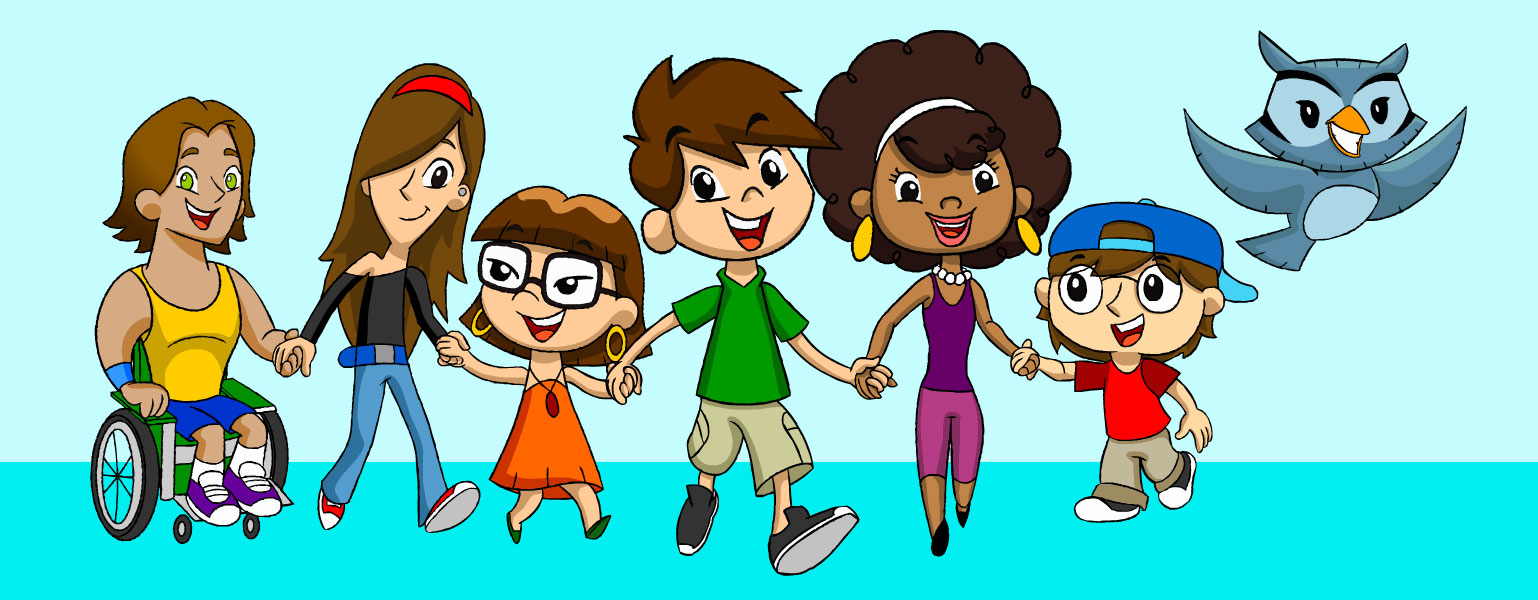
\includegraphics[width=\textwidth]{media/image28.jpeg}

\textbf{Dia Internacional dos Direitos Humanos}


``Todos os seres humanos nascem livres e iguais em dignidade e
direitos. São dotados de razão e consciência e devem agir em relação
uns aos outros com espírito de fraternidade''. Esse é o Artigo I de um
documento muito importante chamado Declaração Universal dos Direitos
Humanos.

O texto é um dos documentos básicos da Organização das Nações Unidas que
faz aniversário dia 10 de dezembro, dia em que a Declaração foi
assinada. Na declaração, são enumerados os direitos que todos os seres
humanos têm, sem distinção alguma, seja de raça, de cor, de sexo, de
língua, de religião, de opinião política ou outra, de origem nacional ou
social, de fortuna, de nascimento ou de qualquer outra situação. E, é
claro, devem ser respeitados por todos.

São direitos básicos para promover a liberdade, a justiça e a paz no
mundo (saúde, educação, cultura e arte, liberdade de informação e
expressão, habitação e alimentação adequadas, entre outros). A
declaração serve como um tipo de guia para que governos, entidades e
cidadãos em cada país respeitem e sejam respeitados, além de inspirar
tratados internacionais sobre direitos humanos.

Talvez você não saiba, mas o francês René Cassin, conhecido como ``o
homem dos direitos humanos'', foi um dos ``pais espirituais'' e redator
principal do primeiro projeto de Declaração Universal dos Direitos
Humanos. Ele perseguiu sem descanso a sua missão internacional de
humanista. Assim, por sua ação em favor do ``respeito aos direitos
humanos no contexto mundial'', recebeu, em 1968, o Prêmio Nobel da Paz.

O Dia Internacional dos Direitos Humanos é mais que uma data
comemorativa. É um momento para que todos lembrem e reflitam sobre a
garantia dos direitos humanos na sua comunidade, cidade, país e em todo
o mundo. O respeito a esses direitos e a garantia de uma vida digna
depende da vigilância e participação de todos os povos e nações.

\textbf{Reconhecimento aos defensores dos Direitos Humanos no Brasil}\\
O respeito aos direitos humanos é condição para o desenvolvimento de
qualquer país. Por isso, aqui no Brasil, institui-se o Prêmio Direitos
Humanos. Ele é a mais alta condecoração do governo brasileiro a pessoas
e entidades que se destacam na defesa e na promoção e também no
enfrentamento e no combate a violações dos direitos humanos no país.

\fonte{DIA Internacional dos Direitos Humanos. Plenarinho. Disponível em:
https://plenarinho.leg.br/index.php/2017/01/dia-internacional-dos-direitos-humanos/. com alterações. 
Acesso em: 25 abr. 2023.}
\end{quote}

\pagebreak
\begin{escolha}
\item Qual é o assunto do texto?

\reduline{O assunto do texto é o Dia Internacional dos Direitos Humanos.\hfill}
\linhas{1}

\item Qual é o Artigo I da Declaração Universal dos Direitos Humanos?

\reduline{``Todos os seres humanos nascem livres e iguais em dignidade e
direitos. São dotados de razão e consciência e devem agir em relação
uns aos outros com espírito de fraternidade''.\hfill}
\linhas{2}

\item Por que René Cassin recebeu, em 1968, o Prêmio Nobel da Paz?

\reduline{René Cassin recebeu o Prêmio Nobel da Paz por sua
ação em favor do ``respeito aos direitos humanos no contexto mundial''.\hfill}
\linhas{3}

\item Segundo o texto, o que é o Prêmio Direitos Humanos?

\reduline{O Prêmio Direitos Humanos é a mais alta
condecoração do governo brasileiro a pessoas e entidades que se destacam
na defesa e na promoção e também no enfrentamento e no combate a
violações dos direitos humanos no país.\hfill}
\linhas{2}
\end{escolha}

\num{2} Nos trechos reproduzidos a seguir, identifique os fatos com \textbf{F}
e as opiniões com \textbf{O}.

%\coment{Antes da realização desta atividade, importante salientar aos alunos que um modo de perceber se alguma informação é um fato ou opinião é observar se ela pode ser comprovada com evidências (no caso do fato) ou se é possível concordar ou não com o que é dito (no caso da opinião).}

\begin{boxlist}
\boxitem{F} ``Todos os seres humanos nascem livres e iguais em
dignidade e direitos. São dotados de razão e consciência e devem agir 
em relação uns aos outros com espírito de fraternidade''

\boxitem{O} ... ``E, é claro, devem ser respeitados por todos.''

\boxitem{O} ... ``A declaração serve como um tipo de guia para que
governos, entidades e cidadãos em cada país respeitem e sejam respeitados,
além de inspirar tratados internacionais sobre direitos humanos''.

\boxitem{O} ... ``Talvez você não saiba, mas o francês René Cassin,
conhecido como ``o homem dos direitos humanos''.

\boxitem{F} ... ``o francês René Cassin, conhecido como ``o homem 
dos direitos humanos'', foi um dos ``pais espirituais'' e redator principal do
primeiro projeto de Declaração Universal dos Direitos Humanos''.
\end{boxlist}

\num{3} Leia o trecho do texto a respeito do Dia Mundial da Liberdade de
Pensamento:

\begin{quote}
\textbf{Dia Mundial da Liberdade de Pensamento}

Pode ser a falta de proximidade, de contato olho no olho; pode ser a
certeza de que não haverá um revide imediato; ou, ainda, a ilusão do
anonimato que a internet proporciona -- o fato é que as pessoas insultam
outras pela web de um jeito que jamais fariam se estivessem frente a
frente. E as redes sociais são o grande palco dessas agressões.

Em todo o mundo, grandes empresas como Facebook, YouTube e Twitter
abriram canais em que os usuários podem denunciar conteúdos e contas que
disseminam ou incentivam a violência. Embora qualquer tipo de agressão
seja passível de punição, há uma que se distingue pela gravidade: é o
discurso de ódio.

O discurso de ódio tem como principal característica o fato de querer
atingir uma minoria {[}...{]} Ele é especialmente nocivo porque promove
a intolerância e impede a pluralidade de vozes, ferindo assim
a democracia. {[}...{]}

Precisamos formar cidadãos que, cada vez mais, saibam que discurso de
ódio não é piada, opinião, polêmica ou controvérsia. Liberdade de
expressão é um direito valiosíssimo, que deve ser usado para fortalecer
a democracia, não para silenciar minorias.

\fonte{DIA Mundial da Liberdade de Pensamento. Plenarinho. Disponível em:
https://plenarinho.leg.br/index.php/2021/07/dia-mundial-da-liberdade-de-pensamento/.
Acesso em: 25 abr. 2023.}
\end{quote}

\begin{escolha}
\item Escreva um trecho do texto que expressa:

%\coment{Ajude os estudantes a diferenciar fato de opinião. Esse tema causa dificulades e dúvidas para eles, mas é fundamental que, de modo gradual, eles se habituem a realizar esse tipo de análise.}

\begin{itemize}
\item o \textbf{fato} que foi noticiado: \reduline{Foi noticiado o Dia Mundial
  da Liberdade de Pensamento e o combate ao discurso de ódio.\hfill}

\item A \textbf{opinião} dos autores do texto: \reduline{Sugestão de resposta:
  Precisamos formar cidadãos que, cada vez mais, saibam que discurso de
  ódio não é piada, opinião, polêmica ou controvérsia.\hfill}
  
\item O \textbf{motivo} da opinião dos autores do texto: \reduline{Liberdade de
  expressão é um direito valiosíssimo, que deve ser usado para
  fortalecer a democracia, não para silenciar minorias.\hfill}
\end{itemize}

\end{escolha}

\colorsec{Treino}

\num{1} Leia o trecho de uma carta do leitor.
%(Fácil) 

\begin{quote}
\textbf{Fogo na Amazônia}

É um absurdo a ineficácia das autoridades responsáveis por esse assunto
{[}\ldots{}{]}. Parecem ignorar que na região o Exército tem Batalhões
de Selva, a Marinha tem embarcações preparadas e batalhões de fuzileiros
navais, e a Força Aérea, aeronaves de patrulhamento para agir de
imediato assim que se detecta o início de um desmatamento ou de um foco
de incêndio.

Com tudo isso, poderiam impedir essas situações e prender os envolvidos.
Mas o resultado aí está, com o fogo atingindo o Pantanal e a fumaça já
chegando até o Rio Grande do Sul.

\fonte{Painel do Leitor. Folha de São Paulo. Disponível em:
https://www1.folha.uol.com.br/paineldoleitor/2020/09/fome-assim-no-brasil-no-seculo-21-e-barbarie-diz-leitor.shtml.
Acesso em: 15 mar. 2023.}
\end{quote}

Com base na leitura da carta do leitor, pode-se identificar que o leitor
quis apresentar

\begin{escolha}
\item uma sugestão para o jornal realizar uma reportagem a respeito do tema.

\item uma opinião sobre uma questão publicada no jornal.

\item uma crítica ao veículo jornalístico sobre a questão da Amazônia.

\item uma pergunta às autoridades sobre a questão da Amazônia.
\end{escolha}

\num{2} Leia um trecho da reportagem a seguir.
%(Médio)

\begin{quote}
\textbf{População brasileira é a 5ª mais feliz do mundo, diz pesquisa}

Os brasileiros nunca foram tão felizes, mas apenas quatro em cada dez
estão satisfeitos com a economia, segundo uma pesquisa do instituto
Ipsos que avaliou a felicidade da população em 32 países.

No Brasil, 83\% dos entrevistados consideram-se muito felizes ou felizes
--- uma alta de 20 pontos percentuais em relação ao último levantamento,
feito em dezembro de 2021, quando o índice foi de 63\%. No mundo, a
percepção de felicidade também subiu, de 67\% para 73\%.

``As pessoas estão vendo este ano como o encerramento de um capítulo
extremamente desafiador em nossa história: a covid-19, ainda que a
pandemia não tenha sido totalmente erradicada, seu impacto é
infinitamente menor do que nos últimos anos. Esse sentimento reforça a
percepção de felicidade'', diz Marcos Calliari, CEO da Ipsos no Brasil.

\fonte{População brasileira é a 5ª mais feliz do mundo, diz pesquisa. BBC
Brasil. Disponível em:
https://www.bbc.com/portuguese/articles/cye4ll78l3wo. Acesso em: 16 mar.
2023.}
\end{quote}

No terceiro parágrafo, o trecho que está entre aspas mostra a

\begin{escolha}
\item opinião do autor da reportagem.

\item opinião do CEO da Ipsos no Brasil.

\item explicação sobre a pesquisa.

\item opinião dos entrevistados.
\end{escolha}

\num{3} Leia o texto a seguir.
%(Difícil)

\begin{quote}
\textbf{'Corvo-Correio', da escritora Isabel Cintra, também foi lançado 
em Angola}

José é um corvo que sonhava voar para entregar cartinhas ao lado dos
pombos brancos. No entanto, o irredutível chefe do serviço postal do
bosque, Coruja Mafalda, não permite. ``Mas você é um corvo! Certamente já
deve ter ouvido dizer que os corvos não servem para carteiros. Todos
sabem disso!'', diz. Após ser praticamente ignorado e rejeitado, José
decide ir embora da região. Mas o jogo vira quando o inverno chega. O
livro infantil \textit{Corvo-Correio} fala sobre valores como tolerância,
igualdade e representatividade, conceitos que precisam ser cada vez mais
trabalhados com os pequeninos.

``O Corvo José é orgulhosamente meu pássaro negro mensageiro. Na
verdade, este protagonista cheio de força sempre esteve presente em
algum lugar em mim, durante toda a minha infância e se escondia
assustado a cada situação de preconceito vivida. Foi preciso uma espera
de crescimento, abandonar o silêncio da criança para deixar a coragem
emergir em forma de palavras que propagam afeto'', explica a autora
Isabel Cintra.

\fonte{\textit{Corvo-Correio}, da escritora Isabel Cintra, também foi
lançado em Angola. Estadão. Disponível em:
https://www.estadao.com.br/emais/comportamento/livro-infantil-traz-licoes-sobre-preconceito-exclusao-e-resiliencia/.
Acesso em: 25 abr. 2023.}
\end{quote}

O trecho em que o autor da reportagem apresenta um fato objetivo sobre
o conteúdo do livro é

\begin{escolha}
\item ``O Corvo José é orgulhosamente meu pássaro negro mensageiro''.

\item ``fala sobre
valores como tolerância, igualdade e representatividade''.

\item ``Na verdade, este protagonista cheio de força sempre esteve
presente em algum lugar em mim''.

\item ``Foi preciso uma espera de crescimento, abandonar o silêncio da
criança para deixar a coragem emergir em forma de palavras que propagam
afeto''.
\end{escolha}

\chapter{Infográficos}
\markboth{Módulo 9}{}

%\coment{Neste módulo, os alunos vão interpretar infográficos, relacionando-os ao contexto em que estão inseridos.}

\conteudo{
\textbf{Infográficos}

%https://www.pexels.com/pt-br/foto/realizacao-conquista-facanha-sucesso-7948039/
\begin{wrapfigure}{l}{.5\textwidth}
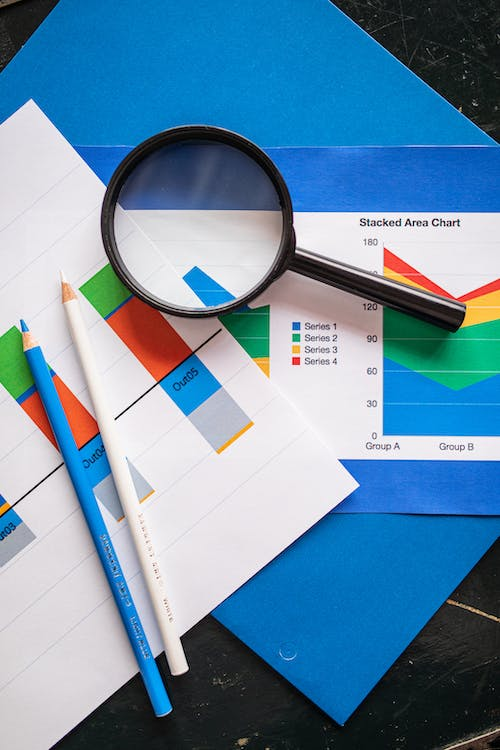
\includegraphics[width=.5\textwidth]{media/image29.jpeg}
\end{wrapfigure}

Infográficos servem para informar ou explicar algo de modo breve,
objetivo, dinâmico e em linguagem acessível por meio de textos curtos
escritos e elementos não verbais. Os temas abordados nos infográficos
costumam tratar das mais diversificadas áreas.

Normalmente, os infográficos podem ser encontrados em revistas, jornais
e \emph{sites} da internet, acompanhando, complementando e/ou resumindo
as informações veiculadas em notícias, reportagens, entrevistas e textos
informativos. Há também infográficos que apresentam as informações sem
fazer parte de outro texto.

Nos infográficos, as informações podem ser apresentadas por meio de
desenhos, fotos, gráficos, tabelas, mapas, cores, formas, entre outros
recursos visuais, e de textos curtos e dados numéricos. Título, imagens 
e legendas são comuns nesses textos.

Os infográficos são exemplos de \textbf{textos multimodais}, isto é,
que apresentam várias linguagens (escrita, visual, verbal).
}

\colorsec{Atividades}

%\coment{Explicar aos alunos que o gráfico deste exercício é conhecido como gráfico de barras. Caso julgue pertinente, mostre aos alunos como se elabora um gráfico usando um programa de computador.}

\num{1} Leia um trecho da notícia a seguir e analise os infográficos,
observando suas funções e as informações apresentadas.

\begin{quote}
\textbf{Recicla Santos quase dobra coleta de recicláveis no último
semestre -- confira infográfico}

%PUBLICADO:~31~DE~JANEIRO~DE~2018~ 18h~20

Coordenador de Políticas Ambientais da Secretaria de Meio Ambiente,
Marcus Fernandes atribui os resultados diretamente ao Recicla Santos.
``Entre junho e julho de 2017, a coleta seletiva passou de 270 para 420
toneladas. Nos 26 anos de história, nunca houve um aumento nessa
dimensão''.

Fernandes lembra que a aplicação do Recicla Santos foi precedida de
palestras, encontros e reuniões realizadas pela Prefeitura para divulgar
a lei entre a população.

Além de aliviar o aterro sanitário do Sítio das Neves, o aumento da
reciclagem traz efeitos positivos para a sociedade e todo o planeta.
``Temos de lembrar, por exemplo, que para se fabricar plástico se gasta
petróleo. A reciclagem reduz a retirada de matéria-prima para a produção
de diversos tipos de produtos. Estamos, assim, utilizando menos água e
energia elétrica''.

O coordenador lembra, ainda, que a nova lei criou postos de trabalho na
área da reciclagem. Atualmente, há duas cooperativas de catadores
atuando na Cidade, a Comares e a Sem Fronteira.

\fonte{Recicla Santos quase dobra coleta de recicláveis
no último semestre -- confira infográfico. Prefeitura de Santos.
Disponível em:
https://www.santos.sp.gov.br/?q=noticia/recicla-santos-quase-dobra-coleta-de-reciclaveis-no-ultimo-semestre-confira-infografico.
Acesso em: 26 abr. 2023.}
\end{quote}

\pagebreak

\begin{figure}[htpb!]
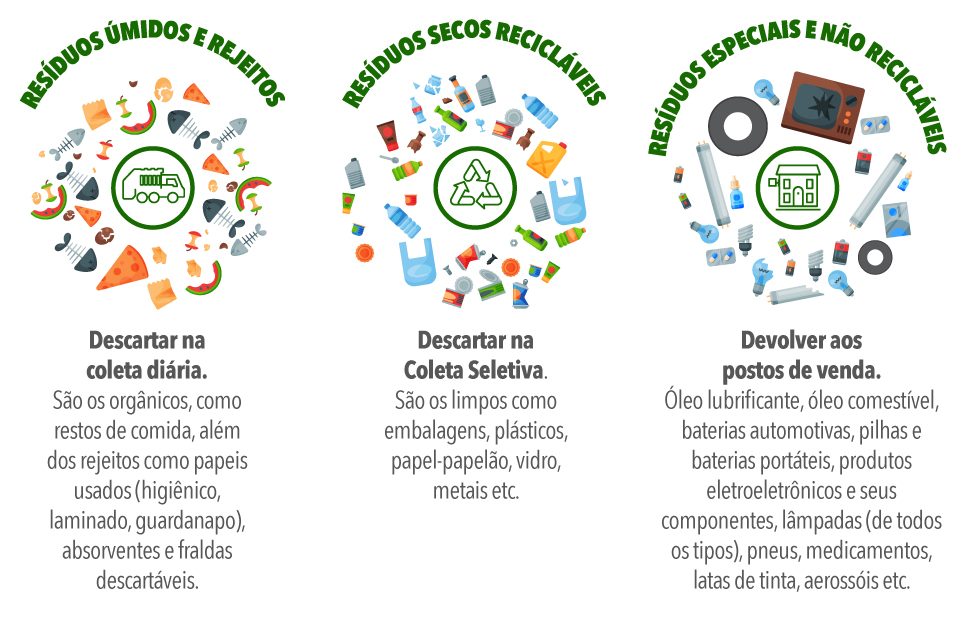
\includegraphics[width=.5\textwidth]{media/image30.jpeg}
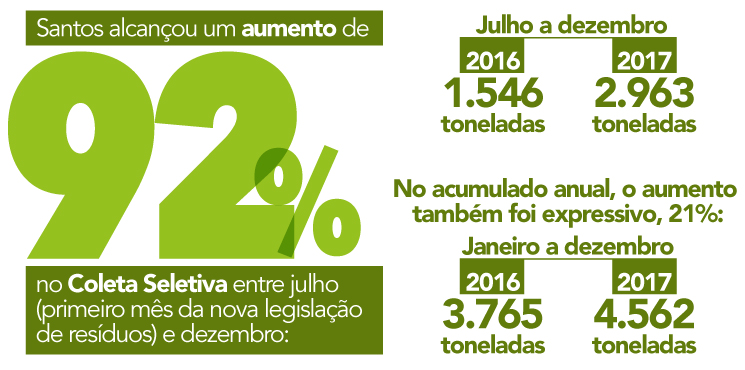
\includegraphics[width=.5\textwidth]{media/image31.jpeg}
\end{figure}

\begin{escolha}
\item Qual é a finalidade desses infográficos?

\reduline{A finalidade dos
infográficos é acrescentar novas informações ao texto verbal, além 
de representar, em linguagem não verbal, o conteúdo dele.\hfill}
\linhas{2}

\item Por que recursos como esse são importantes em textos informativos?

\reduline{Os infográficos e outros recursos similares, como gráficos, 
são importantes porque facilitam a compreensão do conteúdo do texto.\hfill}
\linhas{3}

\item De acordo com o segundo infográfico, qual foi o aumento obtido
pelo Coleta Seletiva entre julho e dezembro?

\reduline{O aumento foi de 92\%.\hfill}
\linhas{1}

\item Qual foi o aumento no acumulado anual?
\reduline{O aumento acumulado anual foi de 21\%.\hfill}
\linhas{1}

\item Marque \textbf{CD} para o que deve descartado na coleta diária,
\textbf{CS} para o que deve ser descartado na coleta seletiva e \textbf{D}
para o que deve ser devolvido aos postos de venda.

\begin{boxlist}
\boxitem{CS} Resíduos limpos.

\boxitem{CD} Resíduos orgânicos.

\boxitem{D} Resíduos especiais.
\end{boxlist}

\item Quantas cooperativas atuam na cidade de Santos? Quais são elas?

\reduline{Há duas cooperativas atuantes em Santos: a Comares e a Sem Fronteira.\hfill}
\linhas{1}

\item Um recurso bastante utilizado em infográficos é a variedade de
tamanhos e cores das letras. Em sua opinião, fazer essa diferença visual
no texto verbal do infográfico é importante? Por quê?

\reduline{Resposta pessoal.
Espera-se que os alunos respondam que esses recursos são utilizados para
destacar elementos que o produtor do infográfico deseja que o leitor
visualize e também para organizar as informações.\hfill}
\linhas{3}
\end{escolha}

\colorsec{Treino}

\num{1} Leia o infográfico a seguir que traz informações relacionadas a
como fazer um clube de leitura.
%(Fácil) 

\begin{figure}[htpb!]
\centering
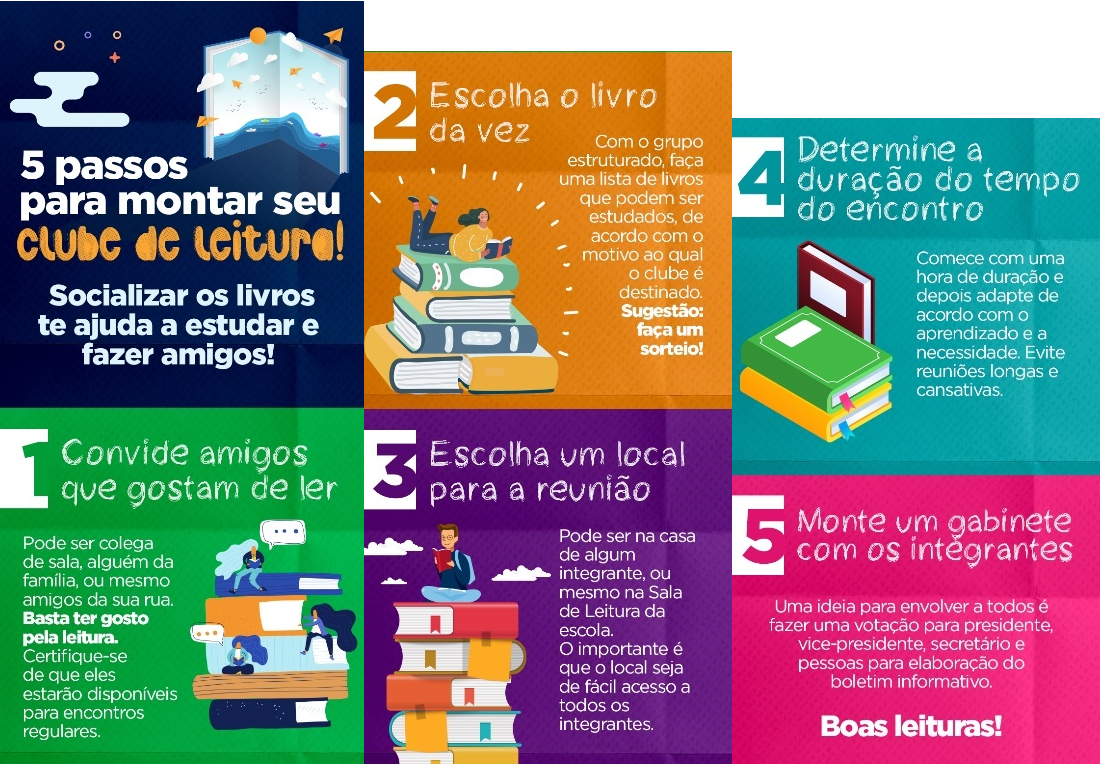
\includegraphics[width=\textwidth]{media/image32.png}
\end{figure}

\fonte{Infográfico: saiba como montar um clube de leitura. Secretaria da 
Educação do Estado de São Paulo. Disponível em:
\textless{}www.educacao.sp.gov.br/noticia/infografico-saiba-como-montar-um-clube-de-leitura/\textgreater{}.
Acesso em: 26 abr. 2023.}

Para organizar as informações nesse infográfico, o autor

\begin{escolha}
\item usou a mesma cor para dividir os itens do passo a passo.

\item escolheu um tipo de letra para cada um dos itens.

\item optou por usar mais imagens e pouco texto.

\item selecionou cores específicas para separar os itens.
\end{escolha}

\pagebreak
\num{2} O infográfico mostra a presença de alunos estrangeiros na rede
estadual de ensino no Estado de São Paulo.
%(Médio) 

%https://www.educacao.sp.gov.br/infografico-alunos-estrangeiros-na-rede-estadual-de-ensino/
\begin{figure}[htpb!]
\centering
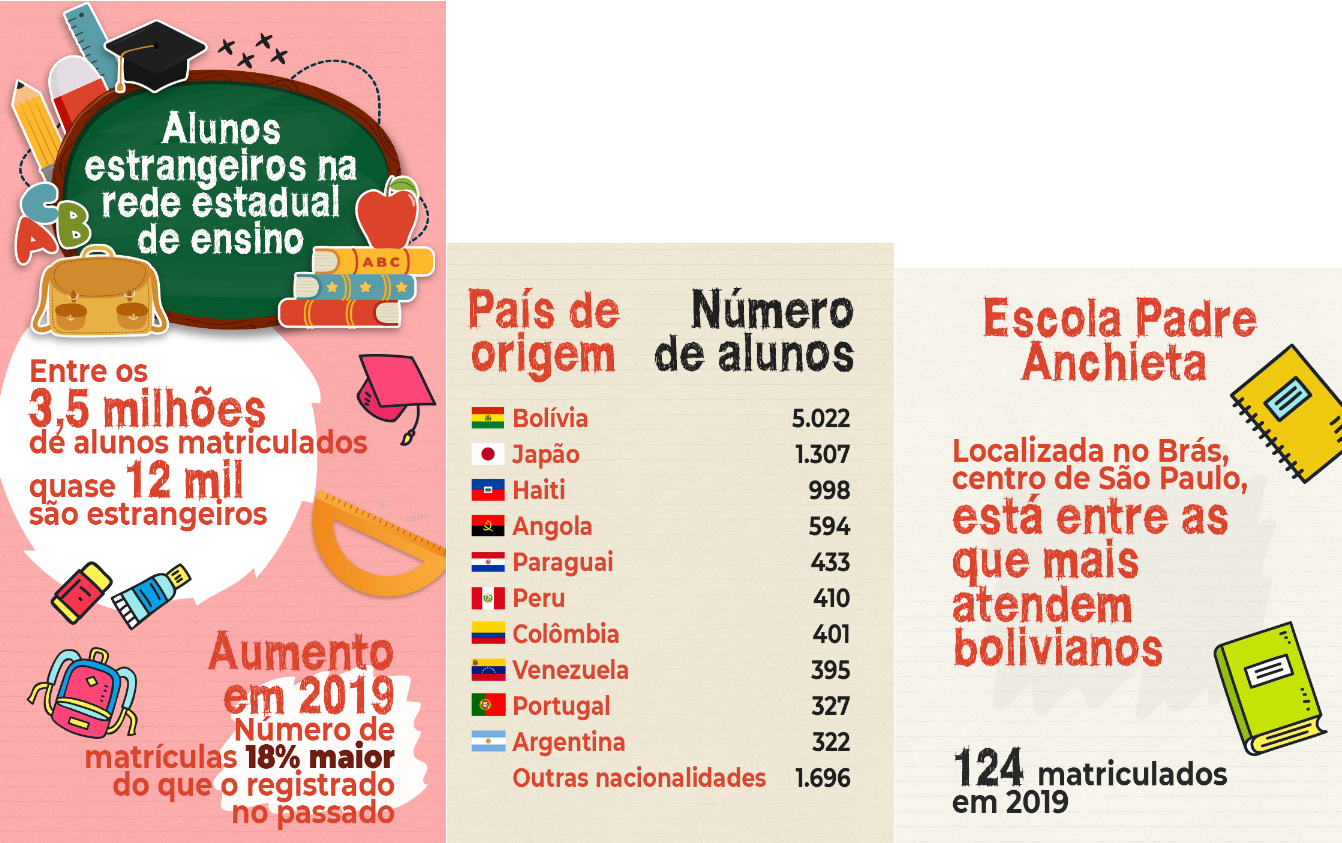
\includegraphics[width=\textwidth]{media/image33.jpeg}
\end{figure}

\fonte{\#Infográfico: alunos estrangeiros na rede estadual de ensino.
Secretaria da Educação do Estado de São Paulo. Disponível em:
www.educacao.sp.gov.br/noticias/infografico-alunos-estrangeiros-na-rede-estadual-de-ensino/.
Acesso em: 18 mar. 2023.}

Podemos observar no infográfico que o número de matrículas em 2019 foi

\begin{escolha}
\item 3,5 vezes maior do que o registrado no ano anterior.

\item 12 mil vezes maior que o registrado no ano anterior.

\item 18\% maior do que o registrado no ano anterior.

\item 124\% maior do que o registrado no ano anterior.

\end{escolha}

\pagebreak
\num{3} Leia o infográfico a seguir.
%(Difícil) 

%www.inca.gov.br/en/node/3201
\begin{figure}[htpb!]
\centering
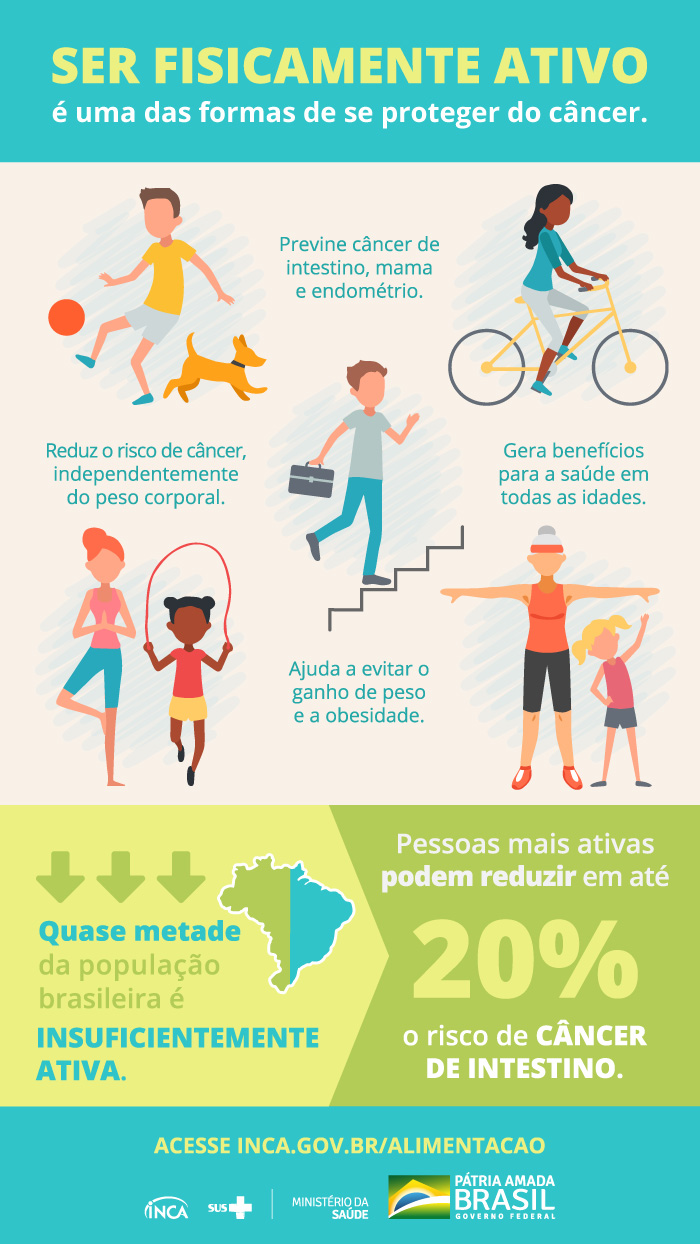
\includegraphics[width=.5\textwidth]{media/image34.jpeg}
\end{figure}

\fonte{Atividade física para o controle do câncer. National Cancer 
Institute. Disponível em: www.inca.gov.br/en/node/3201. Acesso em: 26
abr. 2023.}

Qual é o tema central do infográfico?

\begin{escolha}
\item a população brasileira que é insuficientemente ativa.

\item a atividade física para prevenção do câncer.

\item os malefícios de ser uma pessoa insuficientemente ativa.

\item atividades para prevenção ao câncer de intestino.
\end{escolha}

\chapter{Coesão textual}
\markboth{Módulo 10}{}

%\coment{Nesta seção, os alunos vão analisar palavras utilizadas em trechos de texto para fazer referência aos substantivos; verificar o sentido expresso por essas palavras e observar que estabelecem ligação entre os trechos; identificar os pronomes anafóricos e estabelecer a coesão ao completar trechos com eles.}

%https://www.istockphoto.com/br/foto/bal\%C3\%A3o-de-di\%C3\%A1logo-letras-em-cortar-revista-gm518358614-89988479?phrase=palavras
\begin{figure}[htpb!]
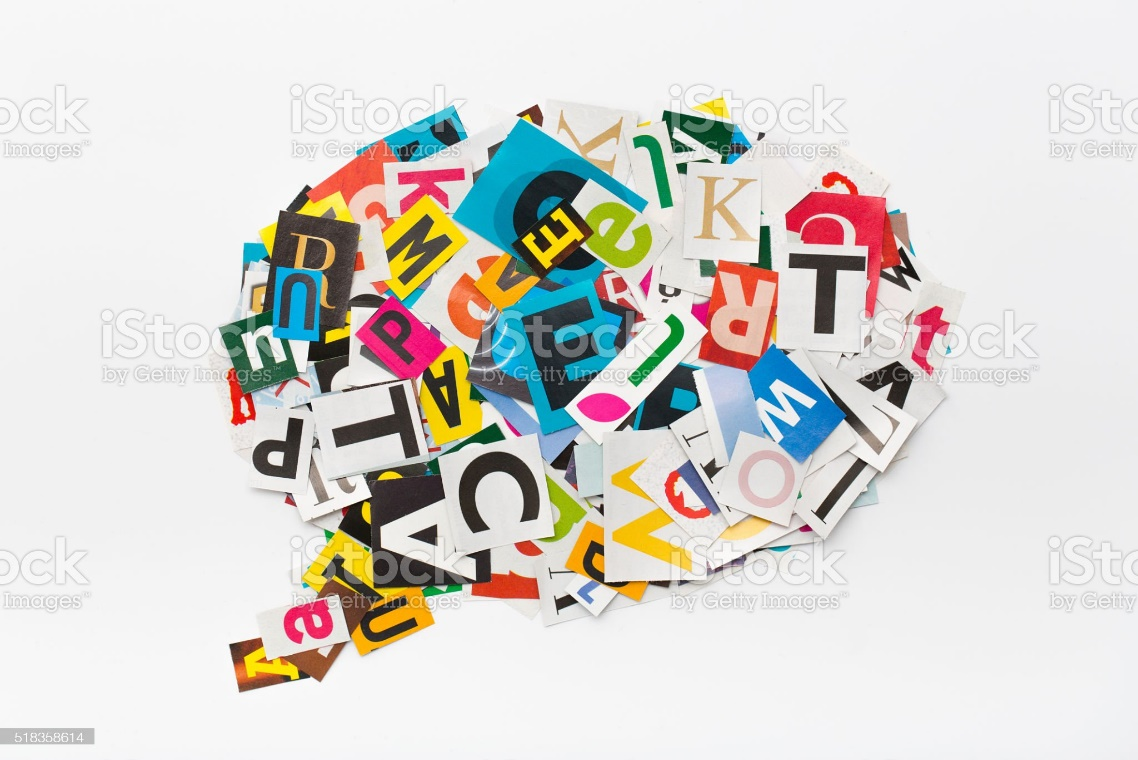
\includegraphics[width=\textwidth]{media/image35.jpeg}
\end{figure}

\conteudo{
\textbf{Coesão}

Na língua portuguesa, há palavras e expressões que podem ser usadas para
ligar as ideias e relacionar os parágrafos, dando progressão ao texto.

\textbf{Coesão} consiste na ligação entre os elementos gramaticais.
Refere-se ao modo como as frases e palavras se relacionam e são
combinadas. A \textbf{coerência}, por sua vez, é a formação lógica 
do texto, o que dá sentido por meio de uma linguagem e sequência 
adequadas. Sem coesão, o texto fica sem qualquer conexão entre as partes;
sem coerência, ele confunde o leitor. Um texto coeso e coerente assegura 
que a sua produção textual cumpra a sua finalidade: comunicar algo,
convencer o leitor ou impactar de algum modo.

Por meio da coesão referencial, cria-se um sistema de relações entre as
palavras e expressões dentro de um texto, fazendo com que o leitor
reconheça os termos aos quais se referem. O termo que indica a entidade
ou situação a que o falante se refere é chamado de referente.
}

\colorsec{Atividades}

\num{1} Leia a narrativa a seguir.

%\coment{Sugere-se propor inicialmente uma leitura silenciosa. Após a leitura, retomar os aspectos que chamaram a atenção de cada aluno. Pode-se fazer, em seguida, uma leitura compartilhada, parágrafo a parágrafo, conversando sobre as palavras desconhecidas e as impressões relacionadas ao texto.}

%https://www.istockphoto.com/br/vetor/ugly-duckling-bullying-concept-vector-cartoon-ilustra\%C3\%A7\%C3\%A3o-gm1372690734-441739165?utm\_source=pixabay\&utm\_medium=affiliate\&utm\_campaign=SRP\_illustration\_sponsored\&utm\_content=https\%3A\%2F\%2Fpixabay.com\%2Fpt\%2Fillustrations\%2Fsearch\%2Fpatinho\%2520feio\%2F\&utm\_term=patinho+feio
\begin{figure}[htpb!]
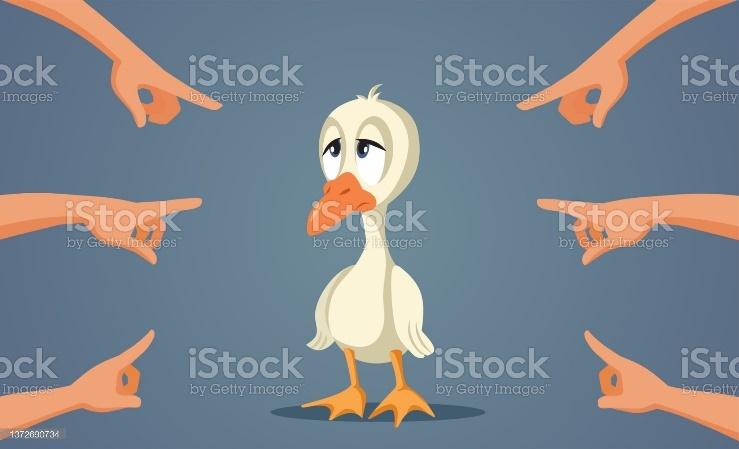
\includegraphics[width=\textwidth]{media/image36.jpeg}
\end{figure}

\begin{quote}
\textbf{O patinho feio}

Em uma bonita manhã de outono, a pata Sofia construiu seu ninho de
gravetos perto do lago. Então passou a chocar. E, depois de trinta e
três dias, cinco de seis ovos se quebraram, e os filhotinhos nasceram
--- todos belos e saudáveis.

Sorrindo, a bicharada foi visitar a mamãe e os bebês:

--- Que lindos patinhos, tão amarelinhos, já aprendendo a nadar. Sejam
bem-vindos!

Mas ainda havia um ovo, que não se abria.

--- Será que não vingará? --- os animais se perguntavam.

Preocupada e esperançosa, Sofia continuou a chocar. Enfim a casca
trincou, e nasceu uma avezinha bem diferente, que não tinha a mesma cor
e graciosidade de seus irmãos. A família achava isso estranho:

--- Quá-quá-quá!

--- Aquele patinho é cinzento!

--- Patinho desajeitado!

--- Patinho feio!

O pobrezinho era sempre excluído, sentindo-se triste e solitário. De
tanto sofrer, resolveu fugir.

Nadou durante todo o dia, em busca de um lar que o acolhesse. Já
anoitecendo, o patinho chegou a uma lagoa cheia de marrecos. Ele se
aproximou e tentou se agrupar. Novamente zombaram dele:

--- Você não pertence à nossa família, pato feio, que não sabe
mergulhar!

Rejeitado, o patinho partiu. Não só nadou, como andou muito. Quando
quase se abeirava de um rio, viu um bando de gansos flutuando sobre as
águas.

--- Eles são cinzas e se parecem comigo. Achei a minha família!

Mas os gansos o expulsaram com ruídos estridentes:

--- Não aceitamos estranhos em nosso lar!

No entanto, o patinho desprezado nunca desistia\ldots{} Enquanto procurava,
ia crescendo e se emplumando. Certo dia, encontrou uma grande lagoa,
onde viviam aves de pescoços longos e sinuosos, de plumas alvas, com
elegância inigualável.

Essas aves foram dóceis com o recém-chegado. Então, ele resolveu ficar
todo o inverno, sendo bem cuidado e amado.

No início da primavera, em uma manhã perfumada pelas cerejeiras, o pato
acordou com um grande alvoroço:

--- Que linda plumagem! Quanta beleza!

Sem acreditar nos elogios, ele olhou para o reflexo na água e se deu
conta de que pertencia àquela família. Na verdade, o patinho feio era um
cisne --- o mais bonito de todos!

\fonte{Hans Christian Andersen. O patinho feio. Disponível em:
https://alfabetizacao.mec.gov.br/images/conta-pra-mim/livros/versao\_digital/o\_patinho\_feio\_versao\_digital.pdf.
Acesso em: 16 abr. 2023.}
\end{quote}

\begin{escolha}
\item De que trata o texto?

\reduline{O texto trata de um patinho que acreditava ser feio até
descobrir que era um belo cisne.\hfill}
\linhas{2}

\item Qual era a cor do último patinho a nascer?

\reduline{Ao nascer, o patinho era cinzento.\hfill}
\linhas{2}

\item O fim da história relata uma descoberta do patinho. Que descoberta
foi essa?

\reduline{O patinho feio descobriu que era um lindo cisne.\hfill}
\linhas{2}
\end{escolha}

\num{2} Releia o trecho a seguir:

\begin{quote}
Nadou durante todo o dia, em busca de um lar que o acolhesse. Já
anoitecendo, o patinho chegou a uma lagoa cheia de marrecos. Ele
se aproximou e tentou se agrupar.
\end{quote}

\begin{escolha}
\item Sublinhe a palavra usada para fazer referência ao patinho feio.

\coment{O aluno deve sublinhar o pronome \textit{ele}.}

\item Por que essa palavra foi usada?

\reduline{O pronome foi usado para substituir o nome patinho, de modo 
a evitar a repetição.\hfill}
\linhas{2}
\end{escolha}

\num{3}

\begin{mdframed}[linewidth=10pt,linecolor=salmao!20,backgroundcolor=salmao!20,roundcorner=20pt]
Nadou durante todo o dia, em busca de um lar que o acolhesse
\end{mdframed}

A palavra \textbf{o} aparece duas vezes nesta frase, com funções diferentes.

\begin{escolha}
\item Qual dessas palavras tem a função de determinar o substantivo \textbf{dia}?

\reduline{O primeiro \textbf{o}.\hfill}
\linhas{1}

\item Qual delas foi usada para substituir a palavra patinho?

\reduline{O segundo \textbf{o}.\hfill}
\linhas{1}
\end{escolha}

\num{4} Quando existe muita repetição em um texto, ele fica com pouca
qualidade. Leia o texto a seguir e observe.

\begin{quote}
O \textbf{Patinho Feio}, na verdade, transformou-se em um cisne
belíssimo. O \textbf{Patinho Feio} ficou muito feliz com essa nova
condição. Os amigos do \textbf{Patinho Feio} fizeram uma grande festa
para homenagear o \textbf{Patinho Feio}. \textbf{O Patinho Feio e seus
amigos} se divertiram muito!
\end{quote}

\begin{escolha}
\item Reescreva o trecho e elimine as repetições que não são necessárias,
mantendo a clareza do texto.

\reduline{Sugestão de resposta: O Patinho Feio, na
verdade, transformou-se em um cisne belíssimo. Ele ficou muito feliz com
essa nova condição. Os amigos dele fizeram uma grande festa para
homenageá-lo. Eles se divertiram muito!\hfill}
\linhas{5}

\item Que alterações no texto você fez evitar as repetições?

\reduline{Foram usados pronomes para evitar repetições.\hfill}
\linhas{1}
\end{escolha}

\num{5} Leia o trecho a seguir e responda: Que pronome pode ser usado 
no trecho para evitar a repetição?

\begin{quote}
Eu, minha mãe e meu irmão assistimos ao filme \textit{O Patinho Feio} na
casa da minha madrinha. \textbf{Eu, minha mãe e meu irmão} adoramos passar
esse tempo juntos.
\end{quote}

\reduline{Nós\hfill}
\linhas{1}

\colorsec{Treino}

\num{1} Leia a charadinha a seguir.
%(Fácil) 

\begin{quote}
Você sabe por que a água foi presa?

Porque ela matou a sede.
\end{quote}

A palavra ``ela'' se refere a

\begin{escolha}
\item ``presa''.

\item ``sede''.

\item ``água''.

\item ``matou''.
\end{escolha}

\num{2} Leia o trecho de uma carta do leitor sobre uma reportagem
publicada na Revista Planeta.
%(Médio) 

\begin{quote}
A reportagem ``Voluntários sem fronteira'' (edição nº 470) me emocionou
do início ao fim devido à riqueza de detalhes e imagens de Moçambique.
Tenho 16 anos e pretendo ser médica. Agora, mais do que nunca, sei que é
essa a profissão que quero para minha vida, para seguir exemplos de
pessoas como os médicos citados na reportagem. Esses profissionais
sacrificam sua vida para ajudar ao próximo e não buscam reconhecimento
ou algo parecido, e sim a valorização da vida de cidadãos que não
possuem ninguém por eles, mas, mesmo assim, ``transmitem a alegria de
viver''.

\fonte{Revista Planeta. Cartas. Disponível em:
www.revistaplaneta.com.br/cartas-29/.  com adaptações. 
Acesso em: 26 abr. 2023.}
\end{quote}

No trecho ``não possuem ninguém por eles'', a palavra ``eles'' se refere
aos

\begin{escolha}
\item ``médicos''.

\item ``cidadãos''.

\item ``profissionais''.

\item ``detalhes''.
\end{escolha}


\num{3} Leia a piadinha a seguir.
%(Difícil) 

\begin{quote}
--- Uma criança vai pela rua com seu avô e encontra um caramelo no chão.
Vai pegá-lo, e seu avô lhe diz: ``não se pega nada do chão''.

Mais adiante a criança encontra uma moeda de um real e seu avô lhe diz:
``não se pega nada do chão''.

Seguem caminhando e seu avô tropeça e cai no chão, e pede ajuda à
criança. E ela lhe diz: ``vovô, não se pega nada do chão''.
\end{quote}

\fonte{Piadas de criança para criança. Guia Infantil. Disponível em:
https://br.guiainfantil.com/piadas-infantis/144-piadas-de-crianca-para-crianca.html.
Acesso em: 26 abr. 2023.}

No trecho ``Vai pegá-lo, e seu avô lhe diz: `não se pega nada do
chão'.'', ``-lo'' está sendo usado no lugar da palavra

\begin{escolha}
\item ``criança''.

\item ``chão''.

\item ``caramelo''.

\item ``avô''.
\end{escolha}

